\documentclass{deliverablereport}

\deliverable{management}{ipr2}
\duedate{31/08/2018 (M36)}
\deliverydate{Unknown}

\usepackage[style=alphabetic,backend=bibtex]{biblatex}
\addbibresource{../../lib/kbibs/kwarcpubs.bib}
\addbibresource{../../lib/kbibs/extpubs.bib}
\addbibresource{../../lib/kbibs/kwarccrossrefs.bib}
\addbibresource{../../lib/kbibs/extcrossrefs.bib}
\addbibresource{../../lib/deliverables.bib}
\addbibresource{../../lib/publications.bib}
% temporary fix due to http://tex.stackexchange.com/questions/311426/bibliography-error-use-of-blxbblverbaddi-doesnt-match-its-definition-ve
\makeatletter\def\blx@maxline{77}\makeatother

\usepackage[show]{ed}
\makeatletter
%%%%%%%%%%%%%%%%%%%%%%%%%%%%%%%%%%%%%%%%%%%%%%%%%%%%%%%%%%%%%%%%%%%%%%%%%%%%%%
% Styling: adapt amsart's subsubsection macro to put a newline after the title
%%%%%%%%%%%%%%%%%%%%%%%%%%%%%%%%%%%%%%%%%%%%%%%%%%%%%%%%%%%%%%%%%%%%%%%%%%%%%%
\renewcommand\subsubsection{\@startsection{subsubsection}{2}%
  \z@{.5\linespacing\@plus.7\linespacing}{.1\linespacing}%
  {\normalfont\bfseries}}

% Variant of taskref that links to the section on the task in this file
\newcommand\localtaskref[2]{\hyperref[#1@#2]{\csname task@#1@#2@label\endcsname}}
\newcommand\longlocaltaskref[2]{\hyperref[#1@#2]{\csname task@#1@#2@label\endcsname: ``\csname task@#1@#2@title\endcsname''}}
\newcommand\longmilestoneref[1]{\textbf{\csname mile@#1@label\endcsname}:
  ``\csname mile@#1@title\endcsname''
  (month \csname mile@#1@month\endcsname)}
\makeatother

%% another level of numbered sectioning
%\usepackage{titlesec}
\setcounter{secnumdepth}{4}

% \titleformat{\paragraph}
% {\normalfont\normalsize\bfseries}{\theparagraph}{1em}{}
% \titlespacing*{\paragraph}
% {0pt}{3.25ex plus 1ex minus .2ex}{1.5ex plus .2ex}

%\usepackage{todonotes}
\author{Nicolas M. Thiéry, Benoît Pilorget, et al.}

\begin{document}
\enlargethispage{4ex}
\maketitle
\githubissuedescription
\tableofcontents\newpage

\section{Explanation of the work carried out by the beneficiaries and Overview of the progress}

In this section, we give a general overview of the progress of the
project during the third reporting period, ranging from September 2018
to August 2019. For new readers, we start by recalling some context of
\ODK's approach that is important to understand and evaluate the
progress; except for the last paragraphs, this piece of text is
unchanged from the preview reporting periods. Then we provide a brief
overview of the work carried out by objective of the project; finally
we detail the progress work package by work package.

\subsubsection*{Some context: \ODK's approach}
\label{section.context}
\ODK's approach to delivering a Virtual Research Environment (VRE) for
mathematics is not to build a monolithic one-size-fits-all VRE, but
rather a toolkit from which it is easy to set up VRE's that are
customised to specific needs by combining the appropriate components
(collaborative workspaces, user interfaces, computational software,
databases, \dots) on top of available physical resources (from
personal laptops to cloud infrastructure). This approach --- chosen by
design --- allows users to flexibly put together lean computational
environments and tools for particular research challenges. These tools
provide the required functionality but due to the component based
approach carry no unnecessary bloat that would reduce effectiveness in
terms of installation process, size, computation time, and
reproducibility.

Most of the components preexist as an ecosystem of open source
software, developed by well established communities of developers. For
example, for interactive computing and data analysis, OpenDreamKit
promotes Jupyter, a web-based general purpose flexible notebook
interface\footnote{a notebook is a document that contains live code,
  equations, visualizations and explanatory text} that targets all
areas of science. A number of Virtual Research Environment already
exist, e.g.\ powered by \cocalc (formerly \SMC) or \JupyterHub.

Hence most of the work in \ODK\ is to foster this ecosystem, improving
the components themselves and their composability. The technical work is
distributed over the work packages:
\begin{itemize}
\item \emph{Component Architecture} (\textbf{WP3}): ease of
  deployment: modularity, packaging, portability, distribution, for
  individual components and combinations thereof; sustainability of
  the ecosystem: improving the development workflows.
\item \emph{User Interfaces} (\textbf{WP4}): enable Jupyter as uniform notebook
  interface, and further improve it; foster the collaboration between
  \cocalc and JupyterHub; generally speaking investigate
  collaborative, reproducible, and active documents.
\item \emph{Performance} (\textbf{WP5}): make the most of available hardware
  (multi-core, HPC, cloud), for individual computational components and
  combinations thereof.
\item \emph{Data/Knowledge/Software} (\textbf{WP6}): enable rich and robust
  interaction between computational components, data bases, knowledge
  bases, and users through explicit common semantic spaces, a language to
  express them, and tools to leverage them.
\end{itemize}
These technical work packages are supported by%
\footnote{The project originally had another work package on
  \emph{Studies of Social Aspects} (\textbf{WP7}); following the
  formal review for reporting period 1, it was decided in agreement
  with the reviewers and advisory board to shut down the work package
  after reporting period 1, moving some of its tasks to other work
  packages, and redirecting the man power for the others to more
  central tasks.}
\begin{itemize}
\item \emph{Community Building and Dissemination} (\textbf{WP2}): developer and
  training workshops, conferences, teaching material with focus on
  making the created value accessible to a wide, varied and growing user community.
\end{itemize}

As a result of \ODK's approach, the work programme for \ODK\ consists
of a large array of loosely coupled tasks, each being useful in its
own right, and none being absolutely critical.

All three reporting periods confirmed that this is a strong
feature of \ODK's approach. Indeed, as analysed in the proposal, this
kind of project is subject to the following risks:
\begin{enumerate}
\item Recruitment of qualified personnel;
\item Different groups not forming an effective team;
\item Implementing infrastructure that does not match the needs of end-users;
\item Lack of predictability for tasks that are pursued jointly with
  the community;
\item Reliance on external software components.
\end{enumerate}
Together with ambitious software challenges, this made the accurate
prediction of workload and precise timeline of work packages
difficult, especially over a period of four years in a field of
rapidly evolving technologies.

And indeed the project actually faced each of the risks above,
especially 1, 4, and 5.
The toughest situation we encountered was the volatility of the personnel at
Sheffield, where the PIs and hired personnel all left for industry at
various stage of the project, some after an intermediate move to
Leeds. However, thanks to the flexibility enabled by
the loose coupling, those risks could be mitigated by adapting the
tasks schedule and human resources allocation, with little influence
on the general aims and objectives.

% The toughest situation we faced was the volatility of the personnel at
% Sheffield, where the PIs and hired personnel all left for industry at
% various stage of the project, some after an intermediate move to
% Leeds. Luckily, most of the work planned for this site was on
% dissemination tasks

OpenDreamKit's approach has one downside: it impedes formal
evaluation, as much for us to assess the adequacy and impact of our
tools, as for our reviewers to assess the depth and value of our
contribution. Indeed, we do not have a main well-defined product and
we capture a very diverse range of end-users and use-cases; hence
quantitative methods of evaluation of the adequacy for end users, like
satisfaction surveys, are rather elusive. In addition, when tools are
jointly developed with the community, how should one attribute the
merit of their success to the project or to the community?

In practice, this certainly added complexity to our reporting efforts
and to our reviewers efforts. It is our \emph{belief} however that
this did not impact the work itself. Indeed, co-design is intrinsic to
the by-users for-users development model of the ecosystem, most of the
participants were also end-users themselves, and we maintained deep
contact with the user community notably through our continuous
dissemination actions. Therefore informal evaluation through first
hand experience or witnessing was largely sufficient to inform the
design and execution of the project.

%  LocalWords:  Jupyter visualizations cocalc composability emph textbf taskref dissem
%  LocalWords:  dissemination-of-oommf-nb-virtual-environment oommf-python-interface hpc
%  LocalWords:  dissemination-of-oommf-nb-workshops oommf-py-ipython-attributes delivref
%  LocalWords:  oommf-tutorial-and-documentation oommf-nb-ve oommf-nb-evaluation 
%  LocalWords:  pythran-typing sage-paral-tree oldpart subsubsection WPtref dksbases

\subsection{Explanation of work carried out per Objective}
%List the specific  objectives  for  the  project  as  described  in  section  1.1  of  Part B   and describe  the  work  carried  out  during  the  reporting  period  towards  the  achievement  of  each listed objective. Provide clear and measurable details.
For reference, let us recall the aims of \ODK.
\begin{compactenum}[\bf {Aim} 1\rm]
\item \label{aim:collaboration} Improve the productivity of
  researchers in pure mathematics and applications by promoting
  collaborations based on mathematical \textbf{software},
  \textbf{data}, and \textbf{knowledge}.
\item \label{aim:vre} Make it easy for teams of researchers of any
  size to set up custom, collaborative \emph{Virtual Research
    Environments} tailored to their specific needs, resources and
  workflows. The \VREs should support the entire life-cycle of
  computational work in mathematical research, from initial
  exploration to publication, teaching and outreach.
  % and bridge the gaps between
  % code, published results, and educational material.
\item \label{aim:sharing} Identify and promote best practices in
  computational mathematical research including: making results easily
  reproducible; producing reusable and easily accessible
  software; sharing data in a semantically sound way; exploiting and
  supporting the growing ecosystem of computational tools.
\item \label{aim:impact} Maximise sustainability and impact in
  mathematics, neighbouring fields, and scientific computing.
\end{compactenum}

Those aims are backed up in our proposal by nine objectives; we now
highlight our main contributions during this reporting period toward
achieving each of them.

\begin{compactenum}[\bf {Obj} 1\rm]
\item\label{objective:framework} \textbf{Virtual Research Environment Kit:} ``\emph{To develop and standardise an architecture
    allowing combination of mathematical, data and software components with off-the-shelf
    computing infrastructure to produce specialised \VREs for different communities.}''

  \ednote{@defeo, @minrk: update for RP3: work carried out for Objective 1: Virtual Research Environment Kit}
  This objective is by nature multilevel; achievements include:
  \begin{itemize}
  \item Collaborative workspaces: major \JupyterHub developments,
    see~\longlocaltaskref{UI}{notebook-collab};
  \item User interface level: enabling \Jupyter as uniform interface for all computational
    components; see \longlocaltaskref{UI}{ipython-kernels}.
  \item Interfaces between computational or database components:
    \begin{itemize}
    \item \emph{short term}: refactoring of existing ad-hoc interfaces, see \longlocaltaskref{UI}{pari-python};
    \item \emph{long term}: investigation of patterns to share data, ontologies, and semantics uniformly across components, see \longlocaltaskref{component-architecture}{interface-systems}, and Section~\ref{dksbases} about \WPref{dksbases}, where we report on the ``Math-in-the-Middle'' (MitM) paradigm for semantic system integration and non-trivial mathematical use cases. In RP3, we have added interoperability of mathematical data sets to the mix. 
  \end{itemize}
\end{itemize}

\item\label{objectives:core} \textbf{Core Components:}
  ``\emph{To develop open source core components
  for \VREs where existing software is not suitable. These components
  will support a variety of platforms, including standard cloud
  computing and clusters. This primarily addresses Aim~\ref{aim:vre},
  thereby contributing to Aim \ref{aim:collaboration}
  and~\ref{aim:sharing}.}''
  \ednote{@defeo, @minrk: update for RP3: work carried out for Objective 2: Core Components
    Presumably we need not list nbval, nbdiff, planetaryum anymore}
  At this stage, it has been possible to implement most of the required developments within
  existing components or extensions thereof. New software components includes the tools
  nbmerge, nbdiff and nbval (see \delivref{UI}{jupyter-test} and
  \delivref{UI}{jupyter-collab}), and planetaryum (see \delivref{dissem}{ils-tool}). For the
  Math-in-the-Middle paradigm for semantic system interoperability we have developed
  knowledge-based Mediator based on the MMT system.
  In RP3 we have concentrated on mathematical data sets. We have added a data aspect to \textsf{MathHub.info} which allows dataset authors to semantically  describe data sets and then generate data database schemata, management functionality, and user interfaces from that. 

\item \label{objective:community}
  \textbf{Community Building across Disciplines:}
  ``\emph{To bring together research
    communities (e.g. users of \Jupyter, \Sage, \Singular, and \GAP) to
    symbiotically exploit overlaps in tool creation building efforts,
    avoid duplication of effort in different disciplines, and share best
    practice. This supports Aims~\ref{aim:collaboration},
    \ref{aim:sharing} and~\ref{aim:impact}.}''
  \ednote{@defeo,@minrk, @ClementPernet: update for RP3: key outcomes of dev workshops
    Maybe: conda packaging, continuous integration}

  We have organized or co-organized a dozen users or developers
  workshops (see~\longlocaltaskref{dissem}{devel-workshops}) which brought
  together several communities. Some key outcomes include:
  \begin{itemize}
  \item Enabling \Jupyter as uniform interface for all computational components; see \longlocaltaskref{UI}{ipython-kernels}.
  \item Sharing best practices for development, packaging, building containers (see~\longlocaltaskref{component-architecture}{mod-packaging}), and continuous integration (see~\longlocaltaskref{component-architecture}{portability});
  \item A smooth collaboration between \JupyterHub, \SMC, and \Simulagora; see~\longlocaltaskref{component-architecture}{extract-smc}, \longlocaltaskref{component-architecture}{simulagora-dev} and Section~\ref{infrastructures};
  \item Work on interfaces between systems; see \longlocaltaskref{component-architecture}{interface-systems}, \longlocaltaskref{UI}{mathhub}, and \longlocaltaskref{UI}{pari-python};
    % \item Steps toward \longlocaltaskref{UI}{sage-sphinx}
  \item Sharing of best practices and tools for authoring live structured documents (see~\longlocaltaskref{UI}{structdocs});
  \item Sharing of best practices when using VRE's like \cocalc or \Jupyter for research and education;
  \item Collaboration on interactive visualization \longlocaltaskref{UI}{vis3d}, \longlocaltaskref{UI}{cfd-vis}, \longlocaltaskref{UI}{dynamic-inspect}.
  \item Jump-starting a community on semantically described, interoperable mathematical data sets around \url{data.mathhub.info}. A Math Data workshop (8 Days) in Cernay included external mathematicians and will be continued by external partners in 2020. 
  \end{itemize}

  \ednote{maybe: mention dissemination workshops as well?}

\item \label{objective:updates}
  \textbf{Updates to Mathematical Software Components:}
  ``\emph{Update a range of existing open source
  mathematical software systems for seamless deployment and efficient
  execution within the VRE architecture of objective~\ref{objective:framework}.
  This fulfils part of Aim~\ref{aim:vre}.}''

  \ednote{@defeo, @ClementPernet: update for RP3: work carried out for Objective 4: Updates to Mathematical Software Components}

  Achievements include:
  \begin{itemize}
  \item Continuous efforts of development, release and integration within \Sage
    have been put for
    \begin{itemize}
    \item  the linear algebra computational kernels of LinBox,
      fflas-ffpack and Givaro (Deliverable~\longdelivref{hpc}{LinBox-algo})
    \item the PARI library for computational number theory
      (Deliverable~\longdelivref{hpc}{pari-hpc2} still ongoing)
    \item the GAP software for computational group theory
      (Deliverable~\longdelivref{hpc}{GAP-HPC-report})
    \end{itemize}
  \item Packaging efforts: docker containers (delivered and regularly
    updated), Debian and Conda packages (beta); see
    \longlocaltaskref{component-architecture}{mod-packaging}.
  \item Continued efforts on portability of \Sage and its dependencies
    (see \longlocaltaskref{component-architecture}{portability}, in
    particular \delivref{component-architecture}{portability-cygwin}).
  \item Improved continuous integration and development workflow;
    (see~\longlocaltaskref{component-architecture}{workflow}), and
    \longdelivref{component-architecture}{multiplatform-buildbot}.
  \item Integration of all the relevant mathematical software in the
    uniform \Jupyter user interface, in particular for integration in
    the VRE framework (delivered, ongoing); see
    \longlocaltaskref{UI}{ipython-kernels}.
  \item Ongoing work in \WPref{hpc} to better support HPC in the
    individual mathematical software system and combinations thereof;
    see Section~\ref{hpc}.
  \item The \Sage and \GAP systems have been extended by a persistent memoization package, which allows to cache computational results and even share them between any system that implementes the memoization format; see \longdelivref{dksbases}{persistent-memoization} for details. 
  \item Ongoing work on the MMT system which forms the basis of the \WPref{dksbases}: Work on \taskref{dksbases}{isabelle} has led to a tight integration with the Isabelle theorem prover and a complete revamp of the code for indexing theory morphisms (crucial for the MitM-based integration of VRE components). 
  \end{itemize}

\item \label{objective:sustainable}
  \textbf{A Sustainable Ecosystem of Software Components:}
  ``\emph{Ensure that our ecosystem of
  interoperable open source components is \emph{sustainable} by
  promoting collaborative software development and outsourcing
  development to larger communities whenever suitable. This fulfils
  part of Aims~\ref{aim:sharing} and~\ref{aim:impact}.}''

  \ednote{@defeo: update for RP3: work carried out for Objective 5: A Sustainable Ecosystem of Software Components
    Maybe: Python 3? phasing out of the Sage notebook? Jeroen's PEP to ease introspection and doctools?
  }

  Achievements include:
  \begin{itemize}
  \item Continued work on outsourcing the computational system user
    interfaces by migrating to \Jupyter; see \longlocaltaskref{UI}{ipython-kernels};
  \item Refactoring \Sage's documentation build system to contribute many local developments
    upstream (\Sphinx) \longlocaltaskref{UI}{sage-sphinx};
  \item Outsourcing and contributing upstream as \Python bindings the existing \Sage
    bindings for many computational systems; see \longlocaltaskref{UI}{pari-python}.
  \end{itemize}

\begingroup
\color{gray}
\item \label{objective:social}
  \textbf{Engineering Social Interactions in Open Source \VRE:}

  This objective was the social science research side of
  \WPref{social-aspects}. Following the work plan revisions after
  Reporting Period 1, the manpower originally allocated to this
  objective was reallocated to other objectives. There thus was no new
  achievements in Reporting Period 2 and 3.

\endgroup

\item \label{objective:data}
  \textbf{Next Generation Mathematical Databases:}
  ``\emph{Identify and extend ontologies and
  standards to facilitate safe and efficient storage, reuse,
  interoperation and sharing of rich mathematical data whilst taking
  account of provenance and citability. This fulfills parts of
  Aims~\ref{aim:vre} and~\ref{aim:sharing}.}''

  This objective is at the core of \WPref{dksbases}; see Section~\ref{dksbases} for details.
  In the first two reporting periods \WPref{dksbases} has developed the Math-in-the-Middle ontology that acts as the pivot point mediating between system languages in the MitM interoperability framework.
  This work has been reported in deliverables \delivref{dksbases}{psfoundation} and \delivref{dksbases}{lfmverif}.

  In the third reporting period the focus of \WPref{dksbases} has been on instantiating the FAIR principles for mathematics (we call the result \textbf{deep FAIR}) and turning mathematical datasets into deep FAIR VRE components.
  This work has been reported in \delivref{dksbases}{nbad-search}.
  The \dmh system, which implements deep FAIR datasets from scratch meets exactly the objectives stated above -- but the system is still very young and needs to attract a critical mass of datasets and community.
  The LMFDB system which has both has been retrofitted with aspects of deep FAIR in \pn, and is much more interoperable than at the start of \pn.
  In parallel, and somewhat dual (lightweight/ad-hoc persistent data caching for mathematical software systems), is the work on \tasktref{dksbases}{data-memo}. Here we have developed a  data memorization format and corresponding memoization packages for \Python (for \Sage) and \GAP.
  These have the potential to lead (by collecting computation results on the side) to informal data sets, which can be semantified later. 

\item \label{objective:demo}
  \textbf{Collaborative Research Environments that Transcend Domains:}
  ``\emph{Demonstrate the effectiveness of Virtual
    Research Environments built on top of \ODK components for a
    number of real-world use cases that traverse domains. This addresses
    part of Aim~\ref{aim:vre} and through documenting best practices in
    reproducible demonstrator documents Aim~\ref{aim:sharing}.}''

  \ednote{@fangohr: update for RP3: work carried out for Objective 8: Collaborative Research Environments that Transcend Domains
    Ubermag's tasks and deliverable
    Shall we mention here other VRE's to illustrate the breath of applications?
    Maybe the interactive text books which cover computer science, biology, physics?
    }

  Most of the work toward this objective is by nature planned for the last period of the \pn
  project. Nevertheless, work has started e.g.  toward the OOMMF demonstrator; see
  \longlocaltaskref{dissem}{dissemination-of-oommf-nb-virtual-environment}
  \longlocaltaskref{dissem}{dissemination-of-oommf-nb-workshops},
  \longlocaltaskref{component-architecture}{oommf-python-interface}.

%Long term sustainability
\item \label{objective:disseminate}
  \textbf{Training and Dissemination:}
  ``\emph{Promote and disseminate
    \ODK to the scientific community by active communication,
    workshop organisation, and training in the spirit of open-source
    software. This addresses Aim~\ref{aim:impact}.}''

  \ednote{@Izabela: update number of meetings and workshops}
  This objective is at the core of \WPref{dissem}, with in particular
  more than 30 meetings, developer, training, and community building
  workshops organized during the third reporting period. See
  Section~\ref{dissem} and \longdelivref{dissem}{workshops-4} for
  details.
\end{compactenum}

%%% Local Variables:
%%% mode: latex
%%% mode: visual-line
%%% fill-column: 5000
%%% TeX-master: "report"
%%% End:

%  LocalWords:  compactenum textbf aim:vre emph JupyterHub longtaskref notebook-collab Simulagora mathhub visualization cfd-vis fflas-ffpack Givaro LinBox-algo multiplatform-buildbot nbad-search dmh psfoundation lfmverif
%  LocalWords:  extract-smc Jupyter localtaskref ipython-kernels dksbases WPref dksbases
%  LocalWords:  nbmerge nbdiff nbval delivref delivref jupyter-collab dissem organized
%  LocalWords:  cocalc portability-cygwin hpc taskref citability fulfills
%  LocalWords:  dissemination-of-oommf-nb-virtual-environment oommf-python-interface
%  LocalWords:  dissemination-of-oommf-nb-workshops

\section{Achievements and ongoing progress in workpackages}
We will now tabulate and explain the achievements of the OpenDreamKit project by the work packages.

\subsubsection{Work Package 1: Project Management}

%Explain, task per task, the work carried out in WP during the reporting period giving details of the work carried out by each beneficiary involved.

%%%%%%%%%%%%%%%%%%%%%%%%%%%%%%%%%%%%%%%%%%%%%%%%%%%%%%%%%%%%%%%%%%%%%%%%%%%%%%
\paragraph{Overview}

As in the previous reporting periods, \site{PS} coordinated \ODK
in close collaboration with the other beneficiaries to ensure that:
\begin{enumerate}
\item{the objectives of the project were met within the agreed budget
    and the timeframe specified by milestones and deliverables;}
\item{all the risks jeopardising the success of the project are managed and that the final results are of high quality;}
\item{the innovation process within the project is fully aligned with the objectives set up in the Grant agreement.}
\end{enumerate}

%%%%%%%%%%%%%%%%%%%%%%%%%%%%%%%%%%%%%%%%%%%%%%%%%%%%%%%%%%%%%%%%%%%%%%%%%%%%%%
\paragraph{Tasks}

\subparagraph{\longtaskref{management}{project-finance-management}}

\begin{itemize}
\item \site{PS} took care of the budget management together with the
  administration body, the D.A.R.I. (Direction des Activités de
  Recherche et de l'Innovation) and its finance service. This included
  prefinancing, interim payments, funds transfer to cater for the moving of personnel
  across sites and from old sites to new sites, and the coordination
  of financial reports.
\item In earlier reporting periods, \site{PS} led four amendment
  processes to the Grant Agreement, to manage work plan revisions and
  to reallocate staff and all remaining resources from the four
  terminated beneficiaries \site{ZH}, \site{USH}, \site{JU},
  \site{USO} to the added beneficiaries \site{UG}, \site{FAU},
  \site{XFEL}, \site{LEEDS}.

  \noindent
  During Reporting Period 3, \site{PS} led a fifth amendment upon
  the request of \site{FAU} to add a subcontractor to conduct a new
  task \longtaskref{dksbases}{isabelle}. Following the suggestions of
  the Project officer, \site{PS} used the occasion to formalize budget
  transfers between beneficiaries to optimize the use of remaining
  resources to achieve the project aims; this was notably required to
  exploit resources left at LEEDS following the early departure of all
  its personnel.

\item In earlier reporting periods,
  \site{FAU} had organized an interim review in Bremen on
  June 2016, and \site{PS} had organized the first
  project review in Brussels on April 2017, and steering committee
  meetings in Orsay (September 2015), St Andrews (January 2016),
  Edinburgh (January 2017), Brussels (March 2017), online (February
  2018), and at \site{XFEL} (June 2018).

  \noindent
  During Reporting Period 3, \site{PS} organized the second project
  review in Luxembourg on October 2018 and steering committee meetings
  in Luxembourg (October 2018) and Marseille (February 2019). It also
  organized a one week "report writing sprint" in Cernay (August 2019)
  to collectively write the project reports. The final review meeting
  will take place in Luxembourg on October 30, 2019, and will gather
  20 \ODK participants to present the project final results.

\item As in earlier reporting periods, \site{PS} ensured that all the
  milestones and deliverables of Reporting Period 3 were achieved
  within its timeframe, and reported on in a timely manner.

\item As in earlier reporting periods, \site{PS} maintained the
  internal and external communication tools that were described in
  \longdelivref{management}{infrastructure}. The project website was
  continuously updated with new content, and virtually all work in
  progress is openly accessible on the Internet to external experts
  and contributors (for example through open source software
  repositories on Github).
  % A new version of the website was released in June 2018.
  % Its end-user friendly interface and content makes it a tool not only
  % for internal communication but very much for dissemination and
  % progress tracking by the reviewers and the community.

\item Concerning the future of \ODK and of its infrastructure toolkit,
  the consortium kept accessing information and getting involved in
  the development of the European Open Science Cloud that is currently
  promoted by the European Commission. The project manager
  participated to the following events:
  \begin{itemize}
  \item \href{https://www.eosc-hub.eu/events/eosc-hub-week-2019}{EOSC
      Hub week}, April 10-12 of 2019, Prague, Czech Republic.
  \item
    \href{https://www.eosc-hub.eu/events/building-open-science-europe-road-ahead-eosc-community}{Building
      Open Science in Europe: The road ahead for the EOSC community
      and the EU Member States}, June 20th of 2019, Tallinn, Estonia.
  \item ICT Proposers' Day 2019, September 19-20th of 2019, Helsinky, Finland.
  \end{itemize}

  \noindent
  In addition, two spin-off proposals were submitted on January 29th
  to the H2020 European E-Infrastructure call INFRAEOSC-02-2019:
  \begin{itemize}
  \item \href{https://github.com/bossee-project/proposal}{BOSSEE}:
    Building Open Science Services on European E-Infrastructure, with
    a focus on Jupyter and applications;
  \item \href{https://opendreamkit.org/2019/01/29/FAIRmat/}{FAIRMAT}:
    FAIR Mathematical Data for the European Open Science Cloud.
  \end{itemize}
  Both were prepared with the same open strategy as OpenDreamKit, and
  involved new combinations of OpenDreamKit and external
  beneficiaries. None was accepted but the respective consortia are
  determined to resubmit them or variants thereof at the earliest
  opportunities.

  % We took advantage of
  % the EOSC stakeholder forum on 28-29 November and the 2017 edition of
  % the DI4R (Digital Infrastructures for Research) in Brussels. During
  % these events we gathered information on the potential of EOSC and
  % how \ODK could fit in there. Furthermore we initiated a partnership
  % with EGI -- a key participant to EOSC -- to deploy \ODK based
  % infrastructure.


\end{itemize}

\subparagraph{\longtaskref{management}{project-quality-management}}

We recall that the Quality Assurance Plan is described in detail in
\longdelivref{management}{ipr}.

\begin{itemize}
% \item Continued success in the recruitment of highly qualified staff.
% \end{enumerate}
\item As in the previous reporting periods, \site{PS} organized the
  interaction with the Advisory Board, composed of seven members, some
  of which specifically represent End Users:
  % The other structure supporting \ODK to ensure the quality of the
  % infrastructure it produce is the Advisory Board. It is
  \begin{itemize}
  \item{Lorena Barba from the George Washington University}
  \item{Jacques Carette from the McMaster University}
  \item{Istvan Csabai from the Eötvös University Budapest}
  \item{Françoise Genova from the Observatoire de Strasbourg}
  \item{Konrad Hinsen from the Centre de Biophysique Moléculaire}
  \item{William Stein, CEO of SageMath Inc.}
  \item{Paul Zimmermann from the INRIA}
  \end{itemize}
  This Advisory Board is composed of academics and/or software
  developers from different backgrounds, countries and communities. It
  is a strong asset to understand the needs of a variety of end-user
  profiles.

\item As in the previous reporting periods, The Quality Review Board
  monitored the quality and the relevance of the software development
  relative to the end-user needs. This board -- chaired by Hans
  Fangohr and composed of four members with a track record of caring
  about the quality of software in computational science -- is
  responsible for ensuring key deliverables do reach their original
  goal and that best practice is followed in the writing process as
  well as in the innovation production process. It met after the end
  of each Reporting Period (RP), and before the Review following that
  RP. More details are given in Section~\ref{section.QAP}.

% More information on
% \longtaskref{management}{project-quality-management} can be found in
% Section 4 of this document: Quality assurance plan.

\item \site{PS} has also been managing risks. Up to the Leeds
  situation, the assessment we present in
  Section~\ref{section.risk_management} has only marginally deviated
  from earlier assessments at Month 12 (\delivref{management}{ipr})
  and Month 36 (\delivref{management}{ipr2}).
\end{itemize}
\subparagraph{\longtaskref{management}{project-innovation-management}}

\begin{itemize}
\item At month 18, \site{PS} had with the help of the consortium a
  first version of Innovation Management Plan
  (\delivref{management}{imp1}), with focuses on:
  \begin{itemize}
  \item{The open source aspect of the innovation produced within \ODK;}
  \item{The various implementation processes the project is dealing with;}
  \item{The strategy to match end-users needs with the promoted VREs}.
  \end{itemize}

  \noindent
  During Reporting Period 3, \site{PS} produced a second version of
  the Innovation Management Plan (\delivref{management}{data-plan2}).
  % to assure that research activities meet the required milestones and
  % produce outputs fully aligned with the project objectives.
  It confirms the elements of strategy of the previous plan, and adds
  two additional sections: one on the choice and impact of open
  licenses in the context of OpenDreamKit, and one on the different
  types of outcome of the project and their respective sustainability.
  This second version also includes minor updates to the earlier
  sections, notably to reflect the work plan revisions that occurred
  after Reporting Period 1.
\end{itemize}

%%% Local Variables:
%%% mode: latex
%%% TeX-master: "report"
%%% End:

%  LocalWords:  subsubsection longtaskref delivref organized Bougeret ipr Csabai
\newpage
\subsubsection{WorkPackage 2:  Community Building, Training, Dissemination, Exploitation, and Outreach}
\label{dissem}
%Explain, task per task, the work carried out in WP during the reporting period giving details of the work carried out by each beneficiary involved.

\ednote{@nthiery, @IzabelaFaguet, @VivianePons: update WP2 for RP3
  - Update T2.1, notably production of comics and videos
  - update the figures in the overview, T2.3, and T2.5; highlight e.g. CIRM
  - ...?
}

%(T2.1, T2.3,T2.5)

During the last period of the project, We  put considerable effort into communicating the outcomes of our work. The major focus of ODK dissemination framework was to ensure that the project’s outcomes  are widely  disseminated  to  the  appropriate  target communities,  and that those communities could contribute to the development process of the further improved mathematical software systems in the spirit of open source; To this end, during the last year of the project, we participated in many dissemination and communication activities through community building workshops.The material we developed for presentation at all our events were made publicly available.

The aim of  task 2.3 was to organize community building development workshops all throughout the project, to bring together developers from the different communities to design and implement some key aspects of OpenDreamKit such as user interface, and documentation and to ensure cross compatibility. For year 4, we have been part of 7 development meetings that gathered not only participants of ODK but also members of the different communities involved. Those were aimed at a specific software componeents(Sage, GAP, SageMathCloud, IPython, Singular, etc.) and to improve joint developments. It fostered collaboration between scientists and developers from different backgrounds to build tools that are needed by all. These workshops were the first step to disseminate our work improving it. 

The second one was to communicate our activities and make them known though the organization of training workshop where anyone interested were welcomed to learn about ODK and see a demonstration of what ODK components can do. One of the main purposes of our disseminative role was to reach these users while fostering diversity. It is in this spirit that we also organized Sage Days to  promote our tools and bring more users and developers from the scientific world. The aim of the T2.5 task was precisely to gather and train more users and foster scientific development around ODK. During Year 4,  one of our main dissemination event was the CIRM conference in Marseille  that welcomed around 50 participants and had a big impact on the scientific community. It brought together users and developers of most ODK software components and consisted of keynote talks and tutorials with a focus on the development of best practices. 
Another important dissemination event was the Sage Days 105, organized as a satellite event to the main yearly international conference  on algebraic combinatorics also involving aroung 50 participants. It featured several tutorials; demos and presentations including best practices. In addition to these events, were organized  our fifth targeted at women event on April 2019 to reduce gender gap in mathematics software developments.  

The impact of development and training workshops was the awareness rising of project results and of the possibilities to strenghten our collaborative open source development model.

Horizontal  activities  were also  implemented  towards  increasing  the  outreach  of  the project  results  and  improving  the  visibility  of  ODK-Eu funded project.

Our communication activities include:
1.	the project’s website
The website for the project has been continuously updated with new content, and virtually all work in progress is openly accessible on the Internet to external experts and.  The   website   is   the   primary   communication   tool   for   dissemination   and communication.  For  this  reason,  it  became  a  repository  for  a  wide  type  of information and communication material and a long-term dissemination and communication tool.

2. Research and Innovation
Micromagnetism Workshop was organized by XFEL on June 2019, to develop a micromagnetic calculator for driving mumax  micromagnetic simulation tool, it was developed as a part of OpenDreamKit project and the advantage is that it allows to run micromagnetic simulations on GPU. Thus could enable us to reach a much larger target audience in the future.

3. Social Media, blogs 
Social media and blogs are good means of outreach to the public and the presence of the project on social networking platform; It has been established from the early stages of the project and used throughout the entire project life, to promote its improvements and results permitting a two-way exchange of information. These tools were used to update on new technical results, and events that might be of interest for our targeted communities, and also to help to share the demos experience, facilitate adoption of project results by the users, to support best practices.  Social media were used also to strengthen the project’s community online and to raise awareness of the project results, as well as  their use and applicability.

4) Press Releases,  comics and  explainer Video
Press Releases were considered an important dissemination and communication tool at the start of the project and will also be at the end. During the very first year, the project has covered six press releases with a general communication about the project.  To promote ODK innovative method and highlight its results to a general public, we plan to submit press releases at the beginning of November, after the Final review meeting. The procedure for the press release production and distribution is still under revision. The text proposal was made available to all the partners  inviting them to finalize its publication through their press offices. The final press releases will be published in French,  the Coordinator’s and 3 partners main language but also translated in English for the others beneficiaries to enable its publication in local media. 
We also plan to send this article proposal to our European communication officer to publish it in the EC newsletter and submit it for publication in the Horizon magazine.  These Press releases will  be  addressed  to   the general press in the high education, research area but also in local press ,  to audiences that do not require a detailed knowledge of the work carried out.  

Also to raise interest of the General public on the project topic and its impact, our communication strategy was accompanied   by   audio-visually   enhanced   materials targeted at non-specialist general public:
-	we authored (with the help of experts) several explainer comics and life and motion-design videos that have been reused in a variety of contexts to promote Binder. % more info needed
-	In  order  to increase  the  visibility  and  public  acknowledgement  of  the  ODK-EU  project,  we created a 2 minutes motion graphic explainer video with Pix Videos, based on the sketches created by Juliette Belin from Logilab.% was published on Youtube?



%%%%%%%%%%%%%%%%%%%%%%%%%%%%%%%%%%%%%%%%%%%%%%%%%%%%%%%%%%%%%%%%%%%%%%%%%%%%%%
\paragraph{Overview}

  We have continued the work started in period one, especially on \longlocaltaskref{dissem}{dissemination-communication} and
  \longlocaltaskref{dissem}{dissemination}, organizing or participating in more than 50 events throughout the last two years.
  In particular, we have intensified our efforts in \textbf{training} the community to use the tools developed through \ODK.
  Indeed we have had 14 workshops or events directly organized by \ODK on subjects such as Jupyter, JOOMF (see \longlocaltaskref{dissem}{dissemination-of-oommf-nb-virtual-environment}), PARI/GP, and more. On top of that, we were also part of 5 SageDays.

  One of our priorities is to increase the diversity of the open-source community in science. We have been organizing
  and supporting initiatives to support women developers and scientists such as: Women in Sage, Code First: Girl, and
  PyLadies. We have also organized specific events in developing countries: Colombia, Mexico, and Morocco.

  Finally, this period was also an occasion to improve our online communication, following the advice of our last review.
  Indeed, we collaborated with students in communication to design a new website. We have also conducted interviews to explain
  the key points of the project and we are working on some multimedia content.


%%%%%%%%%%%%%%%%%%%%%%%%%%%%%%%%%%%%%%%%%%%%%%%%%%%%%%%%%%%%%%%%%%%%%%%%%%%%%%
\paragraph{Tasks}

\subparagraph{\longtaskref{dissem}{dissemination-communication}}
\label{dissem@dissemination-communication}

We have followed the advice from our reviewers and have worked at a better communication:
\begin{itemize}
\item We have worked in collaboration with a master degree in web communication and design. The
\ODK website was the year project of a team of three students who delivered different reports to us, some
new communication ideas and a whole new website design. We implemented the new design ourselves and
organized a small workshop to think as a group about the website organization and content.
\item To reach a wider audience, we decided to use different media for communication. We hired an interviewer
and created short videos to share with our views on project's goals and achievement with our communities. These
video are in final stage of edition and will be released shortly and made available on the website.

\item We have worked with (motion) graphic designers to create
  infographic content for our project. The infography gives a clear
  and fast way to understand the tools we are developing. A first
  sketch illustrating one of our use cases will be posted on the web
  site by the review. More sketches will be posted later this fall and
  will serve as a basis for an explainer video to be produced by
  PixVideos over the winter.
\end{itemize}

\subparagraph{\longtaskref{dissem}{training-portal}}

Training is a core and transversal aspect of our project. It is carried out
through interventions and events as we discuss in \longlocaltaskref{dissem}{dissemination}. These
past two years especially, there is been a very strong effort from the \ODK team to organize
training events and workshops. We are also working on creating better content on our webpage
to help users understand in what aspect of their work can \ODK help. This is why we have create the
``Use Cases'' section.

\subparagraph{\longtaskref{dissem}{devel-workshops}}
\label{dissem@devel-workshops}

Development workshops are a key aspect of OpenDreamKit development model. The aim of these workshops is to bring together developers from the different communities to design and implement some
of the wanted features. As reported in \longdelivref{dissem}{workshops-3}, we have organized
or co-organized 12 of these workshops throughout years 2 and 3 of the project. The thematics varies
for each event: PARI/GP, Linbox, and many cross-thematic events such as GAP-Sage and GAP-Jupyter days,
live structured documents, low level libraries, and more.

\subparagraph{\longtaskref{dissem}{tech-review}}

This task has been started during period one, especially through \delivref{dissem}{techno}. We continue
to keep track of new technologies and report by writing blog posts on our website.


\subparagraph{\longtaskref{dissem}{dissemination}}
\label{dissem@dissemination}

Dissemination is a key aspect of the success of OpenDreamKit. Indeed, our development is carried
out to help and support mathematical communities. One of the goals is to bring
more users and more developers to the different projects we are involved in. The events
that took place during Years 2 and 3 have been reported in \longdelivref{dissem}{workshops-3}.

\begin{compactitem}
\item \textbf{Training workshops and events.} This has been the most important aspect of this task
for the past two years. We have been organizing 14 events covering subjects such as: Jupyter, JOOMMF,
Bioinformatics, HPC, PARI/GP, GAP, experimental mathematics, web data, reproducible workflows.
\item \textbf{Organization of Sage Days in established mathematical communities.} Sage Days have long been
part of the SageMath tradition. By organizing and supporting Sage Days, OpenDreamKit can stay close
the mathematical community, understand its needs, gather more users and developers, and improve
the overall quality of the software. We have been involved in 5 different such events since the beginning
of the project.
\item \textbf{Training activities in developing countries.} \ODK has been present in Colombia for the second time at
the conference ECCO. We also organized SageDays workshops in Mexico and Algeria as well as a PARI/GP event in Morocco.
\item \textbf{Women in \ODK.} Following the organization of Women in Sage in January 2017, two female \ODK participants
have given time and energy to this specific topic. Viviane Pons organized the Women in Sage event, she has also been
an organizer of the \textit{Pyladies Paris} chapter for the last two years. Another Women in Sage is planned for summer 2019. Tania
Allard was a research software engineer for \ODK until July 2018, she worked at the \textit{Code First: Girl} chapter in
Sheffield, and was also invited to the \textit{Diversity and Inclusion in Scientific Computing} event in 2018.
\end{compactitem}

\subparagraph{\longtaskref{dissem}{project-intro}}

\ednote{@mikecroucher, @trallard, @fangohr: proofread brief overview of work done on T2.6: Introduce OpenDreamKit to Researchers and Teachers}

Training and disseminating to Researchers and Teachers is at the heart
of OpenDreamKit and the participants doubled up their efforts during
the last reporting period. This included the organization of training
events (see \longtaskref{dissem}{dissemination} above), but also many
more evaluation and dissemination activities: teaching with
OpenDreamKit technology (thereby training students and other
instructors alike), local consulting, contributing course material and
templates, etc. This is reported on in
\longdelivref{dissem}{IntroODK}, together with some reflection on the
lessons learned at the occasion of these activities: adoption,
adequateness for the needs, best practice.

It should be noted that Sheffield (now Leeds) has been the lead on
this task until its participants got compelling opportunities in the
industry in Fall 2018. This did not reduce the overall dissemination
activities of the project: indeed, the freed resources were
redistributed to other participants that were eager to organize more
activities than originally planned. There was some impact however:
with continued leadership some more of the lessons learned at the
occasion of those activities could have been formally collated, when
currently many are in the state of shared folklore. Luckily this
information is still spreading in the community through many channels:
informal discussions, blog posts, mailing lists, etc.


\subparagraph{\longtaskref{dissem}{dissemination-of-oommf-nb-virtual-environment}}
\label{dissem@dissemination-of-oommf-nb-virtual-environment}

\ednote{@fangohr: update for RP3: brief overview of work done on T2.7, T2.8 micromagnetism VRE}

This task was mostly carried out during the first period. The Ubermag
(previously called JOOMMF) project is working and available on GitHub
(\href{https://github.com/ubermag}{Ubermag repo}). For each Ubermag
package we use continuous integration on both Travis CI and AppVeyor,
where we perform tests and monitor the test coverage, which we then
make available on \href{https://codecov.io/}{Codecov}. Documentation
for each package consists of APIs (automatically generated from the
code) and different tutorials created in Jupyter notebooks. Both of
them are tested on Travis CI. Documentation is built and made publicly
available on \href{http://discretisedfield.readthedocs.io}{Read the
  Docs}. After every major milestone, we upload each package to the
Python Package Index repository and build a Conda package, which can
later be easily installed on different operating systems. We encourage
the early use of our software and invite for feedback for which we
provide several different communication channels. Ubermag can also be
used in the cloud as a Virtual Research Environment, by using Binder
services.

\subparagraph{\longtaskref{dissem}{dissemination-of-oommf-nb-workshops}}
\label{dissem@dissemination-of-oommf-nb-workshops}

We had several workshops and tutorials during major events where we demonstrated the use of our Micromagnetic VRE, received feedback and feature requests from the community:

\begin{compactitem}
\item IOP Magnetism in April 2017, univ. of York.
\item Intermag in April 2017, Dublin.
\item MMM in November 2017, Pittsburgh.
\item Advances in Magnetism in February 2018, Italy.
\end{compactitem}

\subparagraph{\longtaskref{dissem}{ibook}}

In \longdelivref{dissem}{ibook3c} we report on the delivery of two new
open interactive textbooks. Together with the two books delivered
during RP2 (\longdelivref{dissem}{ibook1}), this was the occasions to
explore various approaches to exploit OpenDreamKit technology for
authoring textbooks. In the deliverable report, we reflect on their
respective merits and suggest some best practice.

\subparagraph{\longtaskref{dissem}{index-librorum-salvificorum}} Not
applicable for this period.  The web toolkit \textit{planetaryum}
(\delivref{dissem}{ils-tool}) has been delivered in the 2nd reporting
period, closing the task.

  
%%% Local Variables:
%%% mode: latex
%%% TeX-master: "report"
%%% End:

%  LocalWords:  subsubsection dissem longtaskref organized co-organized longdelivref emph
%  LocalWords:  Jupyter compactitem dissemination-of-oommf-nb-virtual-environment Piwik
%  LocalWords:  delivref centralized cocalc Cython Pythran textbf organizing EuroScyPy
%  LocalWords:  nbgrader nbgrader specialized Codecov joommf-news Micromagnetic Intermag
%  LocalWords:  dissemination-of-oommf-nb-workshops Fruehjahrstagung Sagecell taskref
%  LocalWords:  adcomp index-librorum-salvificorum
\newpage
\subsection{WorkPackage 3:  Component Architecture}
%Explain, task per task, the work carried out in WP during the reporting period giving details of the work carried out by each beneficiary involved.

%%%%%%%%%%%%%%%%%%%%%%%%%%%%%%%%%%%%%%%%%%%%%%%%%%%%%%%%%%%%%%%%%%%%%%%%%%%%%%
\paragraph{Overview}

This Work Package focuses on the structure of the components that make
up a mathematical software and their interactions. Such components can
be separate modules inside a unique software, or separate softwares
interacting through library calls and/or through APIs.

The latest reporting period has focused mainly on improving
development workflows and user experience, in particular targeting
notoriously ``difficult'' platforms such as Windows.

%%%%%%%%%%%%%%%%%%%%%%%%%%%%%%%%%%%%%%%%%%%%%%%%%%%%%%%%%%%%%%%%%%%%%%%%%%%%%%
\paragraph{Milestones} Helping end users perform computations on
whatever hardware they possess is one of the major goals of
OpenDreamKit, and of WP3 in particular. The only milestone involving
WP3 is

\subparagraph{\longmilestoneref{component-architecture-distribution}}

\emph{“User story: users shall be able to easily install ODK's
    computational components on the three major platforms (Windows,
    Mac, Linux) via their standard distribution channels.”}

  With the completion of
  \longdelivref{component-architecture}{portability-cygwin}, all
  OpenDreamKit components now run on Windows. Packages for the major
  Linux distributions (Debian, Ubuntu, Fedora, Arch, ...) have also
  been available for at least a year, thanks to the efforts of the
  community\footnote{Note that the role of OpenDreamKit is to
    facilitate packaging for Linux distributions, by simplifying
    dependency management and build chains, and keeping up to date
    with dependencies. It is not OpenDreamKit's goal to directly take
    the lead on packaging for the dozens of available distributions,
    as this would not be sustainable. We will keep monitoring the
    status of Linux packages, prioritizing more popular distributions
    such as Ubuntu, and continue our efforts to make our components
    easy to package.}. MacOS binaries are regularly released, albeit
  with the usual hiccups typical of the Apple ecosystem.

  The bulk of the milestone is thus completed, ahead of schedule,
  although there is still work to do, the most important items on the
  agenda being better continuous integration, and support for Python 3
  in SageMath\footnote{Python 3 support is vital for SageMath going
    into the year 2020, when Python 2 will be officially
    deprecated.}. We will focus on these items for the remaining year.
  
%%%%%%%%%%%%%%%%%%%%%%%%%%%%%%%%%%%%%%%%%%%%%%%%%%%%%%%%%%%%%%%%%%%%%%%%%%%%%%
\paragraph{Tasks}

  \paragraph{\longtaskref{component-architecture}{portability}}
  \label{component-architecture@portability}
  The first task of this workpackage is to improve the portability of
  computational components.

  The most challenging target is the Windows platform, and indeed
  SageMath has not had native Window support for years. With the
  completion of
  \longdelivref{component-architecture}{portability-cygwin}, we are
  happy to announce Windows support for SageMath: since version 8.0,
  released in July 2017, a one-click installer based on Cygwin is the
  recommended way to install SageMath on Windows. With this
  deliverable, we achieved Windows support for 100\% of OpenDreamKit's
  components.

  In support of developing and maintaining OpenDreamKit's software on
  all platforms, we have also worked on infrastructures for continuous
  integration. No unique solution was found that could accommodate the
  needs of every project, however, through sharing information and
  experience returns, each of the software projects inside
  OpenDreamKit has managed to put in place the infrastructure better
  suited for its needs, leveraging various popular technologies such
  as Docker, Jenkins, etc. These efforts have been reported in
  \longdelivref{component-architecture}{multiplatform-buildbot}.

  \paragraph{\longtaskref{component-architecture}{interface-systems}}
  \label{component-architecture@interface-systems}
  In this task we investigate patterns to share data, ontologies,
  and semantics across computational systems, possibly connected
  remotely.

  The work concerning this work package was essentially completed in
  Year 1, through
  \href{http://www.symbolic-computing.org/science/index.php/SCSCP}{Symbolic
    Computation Software Composability Protocol (SCSCP)}. All
  subsequent planned work has been moved to WP6.

  
  \paragraph{\longtaskref{component-architecture}{mod-packaging}}
  \label{component-architecture@mod-packaging}
  In this task we investigate best practices for composing, sharing
  and interfacing computational components and data for connected
  mathematical systems.

  The main deliverable in this task is
  \delivref{component-architecture}{sage-distribution}, due in month
  48. Thanks to the joint efforts of OpenDreamKit and of the
  community, SageMath is now available as a Debian package, and
  recently also as a Conda package.

  This task is progressing as planned, and we expect to successfully
  complete it next year.

  \paragraph{\longtaskref{component-architecture}{simulagora-dev}}
  The goal of this task is to deliver every six months a new Simulagora
  VM image containing all the software components released over the
  period.

  To this date, five OpenDreamKit VMs have been released in
  Simulagora. The latest version, released in March 2018,
  showcases virtual desktops available from a web browser and
  collaboration workflows based on ``tools'' that can be described as
  micro web applications that require very little development skills
  to set up, but make it easy to make available complex simulations to
  users.
  
  \paragraph{\longtaskref{component-architecture}{component-for-HPC}}
  Not applicable for this period.

  \paragraph{\longtaskref{component-architecture}{extract-smc}}
  \label{component-architecture@extract-smc}
  Recall \cocalc used to be called \SMC at the beginning of this project.
  This task has been terminated early due to the cancellation of
  \longdelivref{component-architecture}{personal-smc}, achieved by the
  \cocalc developers \emph{before the start of \ODK}.

  The resources planned for this task were diverted to other work
  packages.
  
  \paragraph{\longtaskref{component-architecture}{workflow}}
  This task seeks new ways of accepting contributions to mathematical
  software in a scalable way.

  Deliverable \longdelivref{component-architecture}{smc-trac} was
  considerably reshaped to take into account the recent developments
  in the ecosystem. This caused a one year delay in the delivery.

  Thanks to the work done, the entry barrier for developing SageMath
  has been considerably lowered. It is now possible for users with a
  GitHub or GitLab account to contribute to SageMath without having to
  go through a manual (and slow) registration process, and editing
  documentation is now easier then ever, even for the inexperienced
  user.

  With the delivery of
  \delivref{component-architecture}{smc-trac}, this task is now
  complete.

  \paragraph{\longtaskref{component-architecture}{oommf-python-interface}}
  \label{component-architecture@oommf-python-interface}
  Not applicable for this period.

  
%%% Local Variables:
%%% mode: latex
%%% TeX-master: "report"
%%% End:

%  LocalWords:  subsubsection longmilestoneref emph longdelivref portability-cygwin
%  LocalWords:  prioritizing longtaskref multiplatform-buildbot Composability delivref
%  LocalWords:  simulagora-dev Simulagora extract-smc cocalc personal-smc smc-trac
%  LocalWords:  oommf-python-interface
\newpage
\subsubsection{WorkPackage 4: User Interfaces}
%Explain, task per task, the work carried out in WP during the reporting period giving details of the work carried out by each beneficiary involved.

%%%%%%%%%%%%%%%%%%%%%%%%%%%%%%%%%%%%%%%%%%%%%%%%%%%%%%%%%%%%%%%%%%%%%%%%%%%%%%
\paragraph{Overview}

The objective of WorkPackage 4 is to provide modern, robust, and flexible user interfaces for
computation, supporting real-time sharing, integration with collaborative problem-solving,
multilingual documents, paper writing and publication, links to databases, etc. This work is focused primarily around the \Jupyter project, in the form of:

\begin{itemize}
    \item Enhancing existing \Jupyter tools (\localtaskref{UI}{notebook-collab})
    \item Building new tools in the \Jupyter ecosystem (\localtaskref{UI}{notebook-verification}, \localtaskref{UI}{notebook-collab}, \localtaskref{UI}{vis3d})
    \item Improving the use of \ODK components in \Jupyter and \Sage environments (\localtaskref{UI}{ipython-kernels}, \localtaskref{UI}{sage-sphinx}, \localtaskref{UI}{dynamic-inspect}, \localtaskref{UI}{pari-python})
    \item Demonstrating effectiveness of WorkPackage 4 results in specific scientific applications (\localtaskref{UI}{cfd-vis}, \localtaskref{UI}{oommf-py-ipython-attributes}, \localtaskref{UI}{oommf-nb-ve}, \localtaskref{UI}{oommf-tutorial-and-documentation})
    \item Work on Active Documents, which have some goals in common with \Jupyter notebooks (\localtaskref{UI}{structdocs}, \localtaskref{UI}{mathhub})
\end{itemize}

All deliverables for WorkPackage 4 have been delivered and highly successful in previous reporting periods.
There are no new deliverables in Reporting Period 3.
However, the work of software is never really complete.
Work has continued on some tasks to further improve,
mature, and maintain the results of WorkPackage 4
toward sustainability and to best serve \ODK objectives
based on feedback from \ODK and the wider user community.

%%%%%%%%%%%%%%%%%%%%%%%%%%%%%%%%%%%%%%%%%%%%%%%%%%%%%%%%%%%%%%%%%%%%%%%%%%%%%%
\subparagraph{Milestones}

\subparagraph{\longmilestoneref{UI-vre}}

\emph{“The prototype VRE shall be extended with improved ease of deployment, new
  functionality such as interactive 3D visualization and real-time
  collaboration, enabling researchers to collaborate productively in a shared
  computational environment. Finally, integrating notebooks and semantic
  knowledge into a publication / knowledge system enable a continuous process
  of leveraging \ODK components from research to publication.”}


The \Jupyter-based prototype for this has been previously delivered in \longmilestoneref{UI-vre-prototype},
and is extended in \longtaskref{UI}{notebook-collab} to more mature functionality.

WorkPackage 4 has resulted in a number of useful pieces of software
for mathematical researchers,
sometimes creating new software,
improving existing software,
or establishing new or improved connections between two existing systems.

Combining the above, Milestone~\longmilestoneref{UI-vre} has
been reached:
from the obtained toolkit, we can produce a \Jupyter-based VRE,
integrating \ODK components.
The Jupyter kernels delivered in \localtaskref{UI}{ipython-kernels}
enable access to a broader collection of mathematical software.
The interactive utility of software such as \Pari is improved in \localtaskref{UI}{pari-python},
and general interactivity and exploration of mathematical objects in \Sage is improved in \localtaskref{UI}{dynamic-inspect}.
The scope of what classes of work can be made interactive is increased
by the development of interactive three-dimensional visualization tools in \localtaskref{UI}{vis3d}.
Further, the process of collaboration on notebook documents is improved by \localtaskref{UI}{notebook-collab}
and prototype support for live collaboration with \localtaskref{UI}{notebook-collab}.
By focusing on \Jupyter as our User Interface of choice,
all of these tools can be combined in a single VRE,
hosted in the cloud or and made accessible to any researcher,
building on the Docker images created in \longdelivref{component-architecture}{virtual-machines}.

The work in this final reporting period has focused on stabilising and maturing the software delivered in previous periods.

%%%%%%%%%%%%%%%%%%%%%%%%%%%%%%%%%%%%%%%%%%%%%%%%%%%%%%%%%%%%%%%%%%%%%%%%%%%%%%
\paragraph{Tasks}

\subparagraph{\longtaskref{UI}{ipython-kernels}}
\label{UI@ipython-kernels}

All deliverables for this task have been delivered in previous reporting periods.

Kernels for \ODK components \GAP, \Pari, \Sage, and \Singular,
had been delivered in the form of \delivref{UI}{ipython-kernels-basic}
in RP1 and \longdelivref{UI}{ipython-kernels} in RP2.
Work has continued to develop these kernels in this reporting period
to bring them to further maturity and sustainability.

\smallskip
\subparagraph{\longtaskref{UI}{notebook-collab}}
\label{UI@notebook-collab}

All deliverables for this task have been delivered in previous reporting periods.

Prototype components and plan for \delivref{UI}{jupyter-live-collab} had been delivered in RP2.
This has been developed to further complete prototypes of real-time collaboration in JupyterLab in collaboration with the \Jupyter community.
We are optimistic about its completion and adoption in JupyterLab in the near future.
Real-time collaboration has proven to be the largest and most challenging
effort in WP4,
both in terms of technical effort and in community engagement.
The reason being that real-time collaboration needs extensive work
in development in the core of JupyterLab itself,
which required collaboration and coordination with the JupyterLab community for assembling plans and implementation,
aligning with other goals of the JupyterLab project,
including development of new features in the phosphorjs framework on with JupyterLab is based,
and a complete refactor of the JupyterLab data model.
This work has involved participation in workshops and meetings,
as well as addition of \ODK team members to the core JupyterLab team.
As of August 2019, real-time collaboration has been implemented in JupyterLab in a \texttt{datastore} branch on the official jupyterlab repository on GitHub,
and is expected to arrive in a public release of JupyterLab soon.

In addition, further releases of \texttt{nbdime} from
\delivref{UI}{jupyter-collab} have been made
to better support asynchronous collaboration.

This work furthers \ODK objective 5 of promoting sustainable software in math and science.


\smallskip
\subparagraph{\longtaskref{UI}{notebook-verification}}
\label{UI@notebook-verification}

All deliverables for this task have been delivered in previous reporting periods.

\longdelivref{UI}{jupyter-test} was delivered in the form of a new Python package, \texttt{nbval},
which enables testing and verification of existing notebooks via a plugin to the Python testing
framework \textbf{pytest}.
In this reporting period, nbval has received further activity and contributions and new releases.
nbval integrates with nbdime from \delivref{UI}{jupyter-collab} to deliver
testable, reproducible notebooks via traditional software development testing practices.
This work furthers \ODK objective 5 of promoting sustainable software in math and science.

\smallskip
\subparagraph{\longtaskref{UI}{sage-sphinx}}
\label{UI@sage-sphinx}

%%% Updated for RP3 by Jeroen Demeyer %%%
Even though this reporting period contains no explicit deliverables
for this task, significant foundation work was carried out which we
now describe. Documentation tools such as Sphinx rely on introspection
to harvest the documentation out the sources. For performance, a large
fraction of the SageMath sources is however written in Cython
(compiled Python) which, until recently, had an incompatible and
limited introspection API. This forced SageMath and other projects to
maintain bespoke and fragile Sphinx extensions to harvest their
documentation.

Tackling this required to dig deep into the system and design,
implement, and get accepted a change to Python itself: PEP (Python
Enhancement Proposal) 590. PEP 590 makes available Python's fast
calling protocol to custom code, thereby enabling full support for
introspection and documentation to Python functions implemented in C
-- e.g. Cython functions --, with no performance loss. This has been
implemented in the upcoming Python~3.8 and Cython~3.0 releases. We
expect not only Cython and therefore SageMath to benefit from this,
but also other similar projects such as Pythran or Numba.

\smallskip
\subparagraph{\longtaskref{UI}{dynamic-inspect}} Due M36 (\delivref{UI}{ipython-advanced-interacts})
\label{UI@dynamic-inspect}

All deliverables for this task have been delivered in previous reporting periods.

As planned in \delivref{UI}{ipython-advanced-interacts}, \ODK
packages \emph{Sage-Combinat-Widgets} and \emph{Sage-Explorer} were
further developed during RP3.
%
%In versions 0.5.0 to 0.7.6,
\emph{Sage-Combinat-Widgets} has gained in
flexibility and has been applied to a range of new mathematical
objects. User interfaces features like feedback have been enhanced,
and documentation has been augmented and gained a tutorial.
%
%With version 0.5.0,
\emph{Sage-Explorer} has gone through a complete new design and reengineering process,
at the same time for better modularity in the code and for better ergonomics.
%
Finally, the \emph{Francy} Jupyter-based graph visualisation library
was generalized to support \Python -- and therefore \SageMath -- in
addition to \GAP.
%
All three benefited from feedback, if not contributions, from end-users.

% Both build on the robust
% foundation of Jupyter Widgets, and explore what it can bring to
% interactive mathematics. The former focuses on interactive
% visualization and edition of mathematical objects, taking
% combinatorics and discrete math as use case. The latter, which uses
% the former as building block, provides rich, detailed, and efficient
% interactive exploration of objects, their properties and
% interrelations. Both are
% \href{https://github.com/sagemath/sage-explorer}{demonstrated online}
% via the Binder service.


\smallskip
\subparagraph{\longtaskref{UI}{structdocs}}
\label{UI@structdocs}

All deliverables for this task have been delivered in previous reporting periods.

% Active structured documents are a common need with many use cases, and has many potential
% solutions.  Requirements and venues for collaborations were explored through discussions
% between participants, in particular at the occasion of
% \href{https://wiki.sagemath.org/days77/}{Sage Days 77} workshop (see the
% \href{https://wiki.sagemath.org/days77/live-structured-documents}{notes}), and the ODK
% meeting in Bremen. The findings were reported in \longdelivref{UI}{adstex}.

% In \longdelivref{UI}{adcomp}, We have presented a general framework for in-situ computation in active documents. This is
% a contribution towards using mathematical documents -- the traditional form mathematicians
% interact with mathematical knowledge and computations -- as a user interface for a
% mathematical virtual research environments. This is also a step towards integrating the
% two main UI frameworks under investigation in the \ODK project: \Jupyter notebooks and
% active documents -- see~\longdelivref{UI}{adstex} -- at a conceptual level. The system is
% prototypical at the moment, but can already be embedded into active documents via a
% Javascript framework and is ready for use in the \ODK project. The user interface and \SCSCP
% connections are quite fresh and need substantial testing and optimizations.

% \ODK hosted a workshop on live structured documents in October 2017,
% which resulted in the development of \href{https://github.com/minrk/thebelab}{thebelab} software for interactive computing on any website,
% enabling interactivity in traditional web-based documentation,
% and further development of the \MathHub facilities for evaluation in structured documents.

During RP3, we developed the JupyterLab extension
\href{https://gitlab.com/logilab/jupyterhub-training}{JupyterLabTraining}
dedicated to teaching programming, e.g. in Python or Sage.
It provides an environment where learners can autonomously do a
series of exercises in order to learn a new programming language. Each exercise is
an independant Jupyter notebook containing the questions, a cell where the learner will
write her code, a hidden cell containing automated tests, and a button to run these tests
and check the code that has been written answers the questions. The left panel shows
the list of all the exercises; they can be sorted by topic (keyword), complexity or
learning track. Thanks to this environment, each learner can do the exercises at his
own pace and choose the exercises that focus on his own points of interest. The
learning process is thus much more efficient for each person.

We also developed further the
\href{https://github.com/minrk/thebelab}{thebelab} software for
interactive computing in traditional web-based documentation.

\smallskip
\subparagraph{\longtaskref{UI}{mathhub}}
\label{UI@mathhub}

All deliverables for this task have been delivered in previous reporting periods.

One of the most prominent features of a virtual research environment (VRE) is a unified user interface. The \ODK approach is to create a mathematical VRE by integrating various pre-existing mathematical software systems. There are two approaches that can serve as a basis for the \ODK UI: computational notebooks and active documents. The former allows for mathematical text around the computation cells of a read-eval-print loop of a mathematical software system and the latter makes semantically annotated documents active.

\MathHub is a portal for active mathematical documents ranging from formal libraries of theorem provers to informal – but rigorous – mathematical documents lightly marked up by preserving LaTeX markup.

As the authoring, maintenance, and curation of theory-structured mathematical ontologies and the transfer of mathematical knowledge via active documents are an important part of the \ODK VRE toolkit, the editing facilities in \MathHub play a great role for the project,
as delivered in \longdelivref{UI}{mathhub-editing}.

\smallskip
\subparagraph{\longtaskref{UI}{vis3d}}
\label{UI@vis3d}

All deliverables for this task have been delivered in previous reporting periods.

The software developed for this task has been delivered in earlier reporting periods.
Packages such as ipyvolume and k3d-jupyter have received further development,
improved compatibility with JupyterLab,
and developed toward maturity and stability,
with growing community adoption.
Several contributions have been made to JupyterLab and
the \Jupyter ecosystem to further support similar work,
benefiting a wide user community.

\smallskip
\subparagraph{\longtaskref{UI}{cfd-vis}} % M12-36
\label{UI@cfd-vis}

No work to report in this period.


\smallskip
\subparagraph{\longtaskref{UI}{Sage-display}} % M24, no deliverables

No work to report in this period.

\smallskip
\subparagraph{\longtaskref{UI}{oommf-py-ipython-attributes}} % M13-19
\label{UI@oommf-py-ipython-attributes}

The micromagnetic virtual research environment is hosted in the
\Jupyter Notebook. The computational backend is the existing \OOMMF
(Object Oriented MicroMagnetic Framework) simulation tool, which is
accessible through the new Python interface that has been created as
part of \ODK
(\localtaskref{component-architecture}{oommf-python-interface}). The
\Jupyter Notebook allows us to integrate the micromagnetic model
specification, the execution of the simulation, and the postprocessing
and data representation within a single executable document; providing
a new computational research environment for micromagnetic simulation
that uses the most widely used simulation code. We have enhanced this
environment further by exploiting that the notebook allows objects to
represent themselves in different ways within the notebook. For
example, Python objects that represent mathematical equations in the
micromagnetic VRE appear rendered as \LaTeX{} in the notebook. It
allows users to interactively compose and explore computational
models, and to be able to inspect what they have put together in the
language of the scientist (i.e. through equations) rather than through
the language of the computer (i.e. code). The addition of this
representation options does not stop the code from being valid \Python
that can be run outside the notebook. We have also provided a
graphical representation of the mesh and discretisation cell as the
appropriate representation of a finite difference mesh to further
assist the effective communication between code and science user and
graphical representation of vector field objects.  We have used
dissemination workshops to seek feedback from users and to refine
interface.

\smallskip
\subparagraph{\longtaskref{UI}{pari-python}}
\label{UI@pari-python}

No work to report in this period.

% \ednote{@jdemeyer, @videlec: proofread/update report on T4.12: Pari bindings}

% There has been a great deal of progress delivering improved \Pari.
% This work has resulted in benefits to the wider Python and \Sage communities
% via substantial contributions to the \Sage codebase,
% the benefits of which go well beyond this deliverable,
% being used by projects outside \ODK.

% The end results of this first state of the work are the packages
% \href{https://github.com/sagemath/cysignals}{cysignals} and
% \href{https://github.com/defeo/cypari2}{CyPari2}, both installable
% in a pure \Python environment via the standard tool
% \texttt{pip}. Starting from version 8.0, installation via \texttt{pip}
% is \Sage's default way of providing the \Pari interface.

% \longdelivref{UI}{pari-python-lib2} has been delivered, further improving the \Pari packages
% by adding new features, in particular to the Python interface to \Pari.
% \emph{cypari2} has gained the ability produce high-resolution SVG plots.
% It now also supports the dynamic array type from PARI/GP, \verb/t_LIST/.
% The source code of cypari2 is automatically generated.
% This automatic generation has been greatly improved
% and can be re-used outside cypari2 for any Python package that wants to interface efficiently with PARI.
% The cypari2 documentation is also greatly improved,
% as a direct result of improvements to the Sphinx documentation system
% in \localtaskref{UI}{sage-sphinx}.

\smallskip
\subparagraph{\longtaskref{UI}{oommf-tutorial-and-documentation}
  has been merged into
  \longlocaltaskref{dissem}{dissemination-of-oommf-nb-virtual-environment}
}
\label{UI@oommf-tutorial-and-documentation}

\smallskip
\subparagraph{\longtaskref{UI}{oommf-nb-ve}
  has been merged into
  \longlocaltaskref{dissem}{dissemination-of-oommf-nb-virtual-environment}
}
\label{UI@oommf-nb-ve}

%%% Local Variables:
%%% mode: latex
%%% TeX-master: "report"
%%% End:

%  LocalWords:  subsubsection Jupyter taskref notebook-collab ipython-kernels cfd-vis
%  LocalWords:  oommf-py-ipython-attributes oommf-nb-ve oommf-tutorial-and-documentation
%  LocalWords:  mathhub longmilestoneref emph visualization longdelivref UI-vre delivref
%  LocalWords:  jupyter-live-collab ipython-kernel-sage jupyter-collab texttt nbdime
%  LocalWords:  nbval textbf pytest Cython-generated ipython-advanced-interacts adstex
%  LocalWords:  adcomp optimizations thebelab ipyvolume pythreejs threejs ipyscales unray
%  LocalWords:  ipydatawidgets micromagnetic oommf-python-interface cysignals cypari2
%  LocalWords:  dissem dissemination-of-oommf-nb-virtual-environment
\newpage
\subsubsection{WorkPackage 5: High Performance Mathematical Computing}
  \label{hpc}
%Explain, task per task, the work carried out in WP during the reporting period giving details of the work carried out by each beneficiary involved.


  %%%%%%%%%%%%%%%%%%%%%%%%%%%%%%%%%%%%%%%%%%%%%%%%%%%%%%%%%%%%%%%%%%%%%%%%%%%%%% 
  \paragraph{Overview}

  Workpackage 5 is about the development of high performance computing tools in
  mathematical virtual research environments. It is addressed at the level
  of each kernel library composing the computational tools of the project (\Pari,
  \GAP, \Linbox, \MPIR, \Sage, \Singular, ...), and also at the level of interfacing and exposing
  core parallel features to higher level programming interfaces.

  Key results obtained over the period for WorkPackage 5 are the following:
  %% Only list deliverables produced in the reporting period
  \begin{compactitem}
  %% \item A closer integration of \Linbox in \Sage with improved reliability and
  %%   computing efficiency.
  \item A full-featured parallelisation engine, supporting POSIX threads and
  MPI, for PARI in production release of the software
  \item Release of GAP-4.9 allowing compilation  in HPC-GAP compatibility mode.
  %    \item A new super-optimizer for vectorized assembly code and its
  %  exploitation to improve the performances of the MPIR code.
  \item A new symmetric matrix factorization algorithm over finite fields, and
  its high-performance implementation in the \texttt{fflas-ffpack} library.
  \item Major redesign the the polynomial arithmetic used in Singular delivering
  state of the art efficiency.
\end{compactitem}

%%%%%%%%%%%%%%%%%%%%%%%%%%%%%%%%%%%%%%%%%%%%%%%%%%%%%%%%%%%%%%%%%%%%%%%%%%%%%%
\subparagraph{Milestones}

\subparagraph{\longmilestoneref{hpc-prototype}}

\emph{“User story: Astrid wants to run compute intensive routines
    involving both dense linear algebra and combinatorics. She has
    access through a JupyterHub-based VRE to a high end multi-core
    machine which includes a vanilla \Sage installation. She
    automatically benefits from the HPC features of the underlying
    specialized libraries (\Linbox, ...). This is a proof of concept
    of the overall framework to integrate the HPC advances of
    specialized libraries into a general purpose VRE.
    %
    It will prepare the final integration of a broader set of such
    parallel features for the end of the project.”}

With Deliverable~\delivref{hpc}{LinBox-algo}, we developped, released and integrated in the
\Sage the LinBox library and its core dependencies: fflas-ffpack and givaro.
When installing the latest \Sage release on a multithreaded multicore server, it
only takes one configure option to let fflas-ffpack use a multi-threaded BLAS
and therefore expose its parallel speed-up to the end-user of Sage. This feature
is compliant with the use of a higher level of parallelism, through process
workstealing queues that \textit{Astrid} may be using in her combinatorics code, as those
exposed in \delivref{hpc}{sage-HPCcombi}. Now that this first proof of concept has been
successfully achieved, we are working in exposing the more advanced parallel
routines of fflas-ffpack into \Sage, following~\delivref{hpc}{LinBox-DSL}. It
should in particular make Gaussian elimination and related routines enjoy a
better scaling with respect to available CPU cores.

%%%%%%%%%%%%%%%%%%%%%%%%%%%%%%%%%%%%%%%%%%%%%%%%%%%%%%%%%%%%%%%%%%%%%%%%%%%%%%
\paragraph{Tasks}

\subparagraph{\longtaskref{hpc}{hpc-pari}}
Deliverable~\longdelivref{hpc}{pari-hpc1} has been merged
 with \longdelivref{hpc}{pari-hpc2} in the revised workplan.

Deliverable~\delivref{hpc}{pari-hpc2} is on time or even ahead of schedule.
The generic engine for Deliverable~\delivref{hpc}{pari-hpc1} was written and
finalized in 2015 and 2016 and is in production since PARI-2.9 (released
11/2016), it supports sequential evaluation (no parallelism), POSIX threads and
MPI within the same code base.
Development work since then is targeted at using the engine wherever it makes
sense in the code base. The current situation (PARI-2.11, released 07/2018)
includes:
\begin{itemize}
\item fast (near linear time) Chinese remaindering;
\item fast linear algebra over Q and cyclotomic fields, a critical component of
the new "Modular Forms" package;
\item polynomial resultant in $\mathbb{Z}[X]$ via Chinese remainders;
\item computation of classical modular polynomials for about 20 classical
invariants (j, Weber functions, small eta quotients...);
\item discrete logarithm over finite fields (prime fields and
$\mathbb{F}_{p^e}$ for word-sized prime $p$) - polynomial resultant in
$\mathbb{Z}[X] \times \mathbb{Z}[X,Y]$ via 
Chinese remainders / evaluation;
\item APRCL primality proof.
\end{itemize}

More work is underway regarding the development of  ECPP, integer
factorization engines, class group and units computations.

Compared to the pre-existing sequential code, the parallel version adds about 15 extra lines of
C on average (conveniently encapsulated in a separate "worker" object). As usual
in "embarassingly parallel" code, the measured speedup is essentially linear in
the number of available cores. The resulting GP binary has been successfully
crash-tested by a panel of users during the 2017 PARI/GP Atelier in Lyon:
basically, substituting the \texttt{Configure} instruction by \texttt{Configure --mt=pthreads}
before compilation transparently yields the expected speedups for the target
functions on participants dual-core laptops. 


\subparagraph{\longtaskref{hpc}{hpc-gap}}
\label{hpc@hpc-gap}

No deliverable is due for the evaluation period but steady progress was made on
Deliverable~\longdelivref{hpc}{GAP-HPC-report}. Over this period, eight releases were cut
incorporating contributions to Deliverable~\longdelivref{component-architecture}{hpc-configure}.

Another major direction of efforts is the HPC-GAP integration:
HPC-GAP is a fork of \GAP initiated during the \scienceproject project, which
enables multithreaded calculations. Now that HPC-GAP has reached
maturity, it's critical for its widespread use and long term
maintainability to merge it back into \GAP's master branch.
The first step towards this long-standing goal, which is at the core of
Task~\localtaskref{hpc}{hpc-gap}, is the major release of \GAP 4.9, published in 2018 and allowing compilation in HPC-GAP
compatibility mode. It comes together with the new manual book called ``HPC-GAP Reference Manual'',
which is also available online at \url{https://www.gap-system.org/Manuals/doc/hpc/chap0.html}.
HPC-GAP integration required a major
refactorization of \GAP's build system
mainly developed by our external collaborator Max Horn (Giessen) into \GAP's master
branch during the Sage-GAP-Days-85 we organized in March 2017. 
An overview of the most important changes introduced in GAP 4.9.1,
with links to corresponding GitHub entries,
can be found in the \GAP manual: \url{https://www.gap-system.org/Manuals/doc/changes/chap2.html}.
Many \GAP packages also have been updated to work in \GAP 4.9 and make use of its new features.

\subparagraph{\longtaskref{hpc}{hpc-linbox}}
  \label{hpc@hpc-linbox}

The deliverable~\longdelivref{hpc}{LinBox-distributed} due for this reporting period is
delivered on time.

A first focus was made on distributed computing, with an MPI parallelization of a Chinese remainder based
algorihtm. The prototypical implementation first produced was then cleanly integrated in the mainstream code of the
library. Its performance show a very nice scaling with the number of compute nodes on a 256 cores cluster. Although this
approach is best suited for large scale parallelization, its generates a suboptimal workload which become a major
concern on large instances.

An alternative approach based on $p$-adic lifting has an  asymptotically smaller workload, but is intrinsically more
sequential, and therefore less suited for large scale parallelization. 
A major contribution in this task is a new algorithm combining $p$-adic lifting and Chinese remaindering in order to
expose more parallelism without sacrifying the gain in the workload.
We also provide a full-featured  implementation of this new algorithm in \Linbox, which shows delivers both high
efficiency in sequential, and scales well up to 16 cores on a multicore server.

Lastly, we also introduced a support for GPUs in the \texttt{fflasffpack} library and show how matrix product over a finite
field benefit from these accelerators.

All these software improvements are closely integrated in the mainstream code of the \texttt{fflasffpack} and \Linbox libraries.

  \subparagraph{\longtaskref{hpc}{hpc-singular}}
  \label{hpc@hpc-singular}

  The only deliverable under consideration for this reporting period
  is~\longdelivref{hpc}{singular-polyarith}

Multivariate polynomials are represented in Singular using the sdmp format. While this data structure is generally amenable to parallelization, the implementation and some of the algorithms in Singular are not. Since the last update much work has been invested in updating the algorithms and data structures and making Singular polynomial arithmetic competitive with other systems. This work has been done in the Singular submodule Flint, whose code is available at \url{https://github.com/wbhart/flint2}. We also now support polynomial exponents of unlimited size with the three basic monomial orderings of lex, deglex, and degrevlex. Suggestions by colleagues in the HPC community including Bernard Parisse, Michael Monagan, Roman Pearce, and Micka\"el Gastineau have been invaluable.

The serial implementations of the operations of multiplication, division and GCD are complete in both the dense and sparse cases and the performance is competitive with other systems. The parallel implementation of multiplication is also complete with competitive performance as well. We are on track to have division and GCD parallelized and delivered on time.

We have also been able to parallelize polynomial root clustering, which is a
major engine in Singular that benefits from fine-grained
parallelization. Performance improvements continue to be made by Remi Imbach
(now at NYU following his ODK contract). The fully working implementation is
at \url{https://github.com/rimbach/Ccluster}.




  \subparagraph{\longtaskref{hpc}{hpc-mpir}}
  \label{hpc@hpc-mpir}

  Not applicable for this period.
  
  \subparagraph{\longtaskref{hpc}{hpc-combi}}
  \label{hpc@hpc-combi}

  Not applicable for this period.


  \subparagraph{\longtaskref{hpc}{pythran}}
  \label{hpc@hpc-pythran}
  Not applicable for this period.

%%   The goal of this task is to make Pythran easily integratable in large-scale
%%   project, taking into account native dependencies, compilation time, memory
%%   footprint, speed and size of compiled binaries as well as multi-platform
%%   support. Integration with \software{cython} is a possible mean to achieve
%%   this goal.

%%   Two projects have been selected for this task: \software{scipy} and
%%   \software{scikit-image}. These projects are relevant for \software{pythran}
%%   because they have many small to medium kernels that can benefit from
%%   compilation. Even though \software{pythran} has not been selected as a scipy
%%   backend, the exchanges with the community have led to a great deal of
%%   improvements of which all \software{Pythran} users take advantage.  The
%%   \software{scikit-image} community is still examining the possibility of using
%%   \software{pythran} as an acceleration mean.

%%   Integration of  \software{pythran} as a \software{cython} backend for
%%   \software{numpy} has improved in various aspects: better error detection,
%%   more supported expression patterns and improved performance for the compiled
%%   expressions.

%% Deliverable~\longdelivref{hpc}{sage-HPCcombi} is shared with
%% Task~\longlocaltaskref{hpc}{hpc-combi}, the status of which we reported on above.

  \subparagraph{\longtaskref{hpc}{hpc-jupyter}}
  \label{hpc@hpc-jupyter}
  
%% It is common for academic High Performance Computing (HPC) clusters to make
%% use of schedulers based on Sun Grid Engine with Son of Grid Engine as one of
%% the most popular. It is used, for example, on the institutional HPC systems
%% in the Universities of Sheffield and Manchester in the United Kingdom. It is also used
%% on the regional N8 HPC facility, a system shared by the eight most research
%% intensive universities in the North of England.
  Not applicable for this period.

%  LocalWords:  subsubsection hpc compactitem super-optimizer vectorized factorization
%  LocalWords:  texttt fflas-ffpack longmilestoneref emph JupyterHub-based specialized
%  LocalWords:  longtaskref longdelivref delivref finalized mathbb embarassingly taskref
%  LocalWords:  scienceproject refactorization organized LinBox-algo DumPerSul:fcrpmgbd16
%  LocalWords:  Pernet:cqm16,PerSto:tsegqm17 DumKalTho:lticmpdsm16,DumLucPer:cftearp17
%  LocalWords:  Cython Hongguang singular-polyarith sdmp parallelization deglex degrevlex
%  LocalWords:  Monagan Micka parallelized parallelize Imbach hpc-mpir sage-paral-tree
%  LocalWords:  Cilk libsemigroup optimized pythran integratable scipy scikit-image numpy
%  LocalWords:  sage-HPCcombi hpc-jupyter
\newpage
\subsubsection{WorkPackage 6:  Data/Knowledge/Software-Bases}\label{dksbases}
%Explain, task per task, the work carried out in WP during the reporting period giving details of the work carried out by each beneficiary involved.

%%%%%%%%%%%%%%%%%%%%%%%%%%%%%%%%%%%%%%%%%%%%%%%%%%%%%%%%%%%%%%%%%%%%%%%%%%%%%%
\paragraph{Overview}

In a series of workshops (September 2015 in Paris, January 2016 in St. Andrews, June 2016 in Bremen, and July 2016 in Bia{\l}ystok, 2017 in Orsay, 2018 in Cernay, 2019 in Cernay), the participants working on \WPref{dksbases} met and discussed the topic of integrating the \pn systems into a mathematical VRE toolkit.
Additionally, Florian Rabe was employed at both FAU and UPSud throughout 2018 and 2019 to deepen the integration.

Key results of the first two reporting periods were
\begin{compactitem}[\bf R1.]
\item the observation that \emph{knowledge-aware interoperability of software and database-systems is the most critical objective} for \WPref{dksbases} in the \pn project.
\item the consensus that this can be achieved by \emph{aligning the mathematical knowledge underlying the various systems},
\item the existing integration of mathematical computation systems in the Sage and Jupyter systems must be complemented with a similar integration of mathematical databases.
\end{compactitem}
This requires explicitly representing the three aspects of math VREs -- Data (D), Knowledge (K), and Software (S) -- and basing computational services and inter-system communication on a joint \DKS-base.
These results are engrained in the ``Math-in-the-Middle'' (MitM) paradigm~\cite{DehKohKon:iop16}, which gives a representational basis for specification-based interoperability of mathematical software systems -- so that they can be integrated in a VRE toolkit.
In the MitM paradigm, the mathematical knowledge underlying the VREs (K) and the interface for each system (S) are represented as modular theory graphs in the OMDoc/MMT format.
For the data aspect (D) we have extended the concept of OMDoc/MMT theories to ``virtual theories'' that allow the practical management of possibly infinite theories, see~\cite{ODK-D6.5} for details.

Through the concerted effort of the WP6 participants, we have been able to implement this design and instantiate it with generate theory graphs for the \GAP and \Sage systems and integrating the \LMFDB (see~\cite{ODK-D6.5}.
Based on this, we were able to generically integrate \GAP, \Sage, and \LMFDB via the standardised SCSCP protocol~\cite{HorRoz:ossp09}. This case study shows the feasibility of the design. 

\begin{wrapfigure}r{6cm}\vspace*{-1em}
\documentclass{standalone}
\usepackage{tikzinput}
\begin{document}
\providecommand\myscale{4.5}
\begin{tikzpicture}[scale=\myscale]
  \node (center) at (0,.15) {Organization};
  \node (left) at (.2,-.3) {Computation};
  \node (right) at (.4,0) {Tabulation};
  \node (back) at (-.5,0) {Inference};
  \node (up) at (0,.5) {Narration};

  \draw[very thick] (center) -- (left);
  \draw[very thick] (center) -- (right);
  \draw[very thick] (center) -- (back);
  \draw[very thick] (center) -- (up);
  \draw[dotted] (left) -- (right) -- (back) -- (left);
  \draw[dotted] (up) -- (left);
  \draw[dotted] (up) -- (right);
  \draw[dotted] (up) -- (back);
\end{tikzpicture}
\end{document}
%%% Local Variables: 
%%% mode: latex
%%% TeX-master: t
%%% End: 
\vspace*{.5em}
\caption{Five Aspects of Math VREs, a Tetrapod Structure}\label{fig:tetrapod}\vspace*{-1.5em}
\end{wrapfigure}
In the \textbf{third reporting period}, the focus was on the \textbf{representation and curation of mathematical data}, building on the earlier work. We have refined the original notion of \DKS-bases from the grant proposal into a tetrapodal structure which captures the four primary aspects of ``doing Maths'' that have to be supported in a VRE toolkit: narration (papers and textbooks), computation (algorithms and software), inference (theorems and proofs), and tabulation (database schemas and datasets).
These are joined via a fifth modular organization aspect -- see the introduction  of \cite{ODK-D6.10} and \cite{CarFarKohRab:bmobb19} for a discussion.

We have taken up the general discussion of research data, the FAIR principles, and have adapted them to the case of mathematical research data. The outcome of this was the observation that -- even though mathematics deals with ideal and abstract objects -- it is often possible to describe these objects concisely by representing them as database structures in a way that complements they their formal symbolic descriptions. The codecs from the ``virtual theories'' approach developed in \WPref{dksbases} tie these two representations together: they link the database level of mathematical data sets with the MitM ontology -- and from there via the interface theory graphs interface it to the mathematical software systems in \pn.

We undertook three larger case studies to bring this about:
\begin{itemize}
\item developing the system data.mathhub.info for managing mathematical data sets MitM-style and equipping it with a search UI; see the report on \taskref{dksbases}{data-LMFDB} below,
\item exporting a the Isabelle knowledge base (via a subcontract), and equipping it with a semantic search facility; see the report on \taskref{dksbases}{isabelle} below,
\item extending the formula search capabilities developed in the first reporting period to Jupyter notebooks; see the report on
 \taskref{dksbases}{mws} below.
\end{itemize}
This wraps up and integrates the work in \WPref{dksbases} combining aspects of Data (D) (now captured by tabulation), Knowledge (K) (now captured by organization and inference), and Software (S) (now captured by computation).
Importantly, the joint system addresses semantically the central aspects of all four FAIR requirements for the open sharing of research data. 
For a joint and integrated final report on this, see ~\cite{ODK-D6.10}.


%%%%%%%%%%%%%%%%%%%%%%%%%%%%%%%%%%%%%%%%%%%%%%%%%%%%%%%%%%%%%%%%%%%%%%%%%%%%%% 
\paragraph{Milestones}

% month 36
\subparagraph{\longmilestoneref{dksbases-interop1}}
This milestone was addressed in the second reporting period.
\medskip
%\emph{“User story: thanks to a fully functional prototype integrating of at least the systems \GAP, \Sage, \Singular, and \LMFDB via the \SCSCP Protocol, end users shall be able to run calculations involving any combination of those systems from any of them.
%  This prototype will be the basis for integration work for additional systems and the user interface from WP4.”}
%\medskip
%
%Workpackage \textbf{WP6} is fully on track with this milestone.
%After first integration and DKS prototypes (the MitM VRE middleware  framework) became available in late fall 2017 (see~\cite{KohMuePfe:kbimss17,WieKohRab:vtuimkb17}) we were able to develop more sophisticated -- and mathematically more realistic/relevant -- use cases~\cite{CreLow:mdcmds18} and generalize those parts of the framework that had been overly specific to the first use cases.
%This involved non-trivial investments in all parts of the framework, as well as the system API theory generation systems and (in particular) the MitM ontology. 

% month 42
\subparagraph{\longmilestoneref{dksbases-interop2}}
\emph{“The goal of this milestone was to take into account all the operational experiences with the first prototype and add more systems and integrate some of the UI components from WP4.
  The experiences with the preparation of this prototype allow us to estimate the joining costs of adding a system to the OpenDreamKit VRE toolkit, which is an important measure of the flexibility of the Math-In-the-Middle approach.”}

The state of the MitM VRE middleware is sufficiently mature that most of the functionality can be configured by writing domain and system knowledge in form of OMDoc/MMT theories, but without requiring extensions of the system (e.g., changes to the programming of the VRE systems or the MMT mediator).
This means that additional computational systems can be added at the cost of generating system API theories, extending the MitM ontology, and supplying alignments.

In the \emph{third review period} we have concentrated on mathematical data sources.
Our analysis of systems in \taskref{dksbases}{data-OEIS}, \taskref{dksbases}{data-findstat}, and even more \taskref{dksbases}{data-LMFDB} has revealed that to achieve deep and meaningful FAIRness of mathematical research data -- in particular of interoperability (I) -- we have to semantically model the mathematical objects in math-aware representations (as described above).
As a consequence, we have to integrate mathematical data systematically into the \pn VRE toolkit, giving rise to the refined tetrapodal model described above. In particular, this integration must consider individual datasets rather than dataset-related systems like OEIS, FindStat, or LMFDB.
The \dmh system was expressly designed to do this: we can just specify a dataset in the MDDL language (see~\cite{BerKohRab:tumdi19,ODK-D6.10}) and then generate a database infrastructure including user interface and import facility from it, resulting in a MitM-Interoperable VRE component for that dataset.
We have tested and evaluated this setup on a special Math Data Workshop~\cite{ODK-WDM19} using five data sets supplied by one internal and two external mathematicians.
This showed that -- after a learning period of a day and with some help from \pn knowledge engineers, external users can MitM-integrate datasets by specifying their structure and semantics and supplying them in a specification-conforming format in under a day of work.
We anticipate that creating the alignments (see \cite{ODK-D6.5}) that relate the mathematical background of these datasets to algorithms in computational MitM systems like \GAP, \Sage, and \Singular is of the same order of magnitude. 


%%%%%%%%%%%%%%%%%%%%%%%%%%%%%%%%%%%%%%%%%%%%%%%%%%%%%%%%%%%%%%%%%%%%%%%%%%%%%% 
\paragraph{Tasks}
\medskip

\subparagraph{\longtaskref{dksbases}{data-assessment}}
\label{dksbases@data-assessment}
This task was addressed in the first reporting period.
\medskip

\subparagraph{\longtaskref{dksbases}{data-triform}}
\label{dksbases@data-triform}
This task was addressed in the first reporting period.
%For this task we have specified and implemented the concept of virtual theories that can contain large -- theoretically even infinite -- numbers of declarations and objects (e.g. 3.5M declarations in the LMFDB data base for elliptic functions) in OMDoc/MMT.
%Virtual theories are characterized by the fact that they are too large to keep in main memory of the MMT System and have to be partially and lazily imported from an external data store.
%We have reported on the design in \longdelivref{dksbases}{design}, on a first implementation on the international conference (MACIS 2017)~\cite{WieKohRab:vtuimkb17}, and finally on an extended use-case in \LMFDB in \longdelivref{dksbases}{psfoundation}. 
\medskip

\subparagraph{\longtaskref{dksbases}{data-design}}
\label{dksbases@data-design}
This task was addressed in the first reporting period.
%This task was directly addressed in the \WPref{dksbases} workshops in the first year and has led to the design and implementation in \delivref{dksbases}{design}. A first implementation has been presented on the international conference (MACIS 2017)~\cite{WieKohRab:vtuimkb17}, and finally on an extended use-case in \LMFDB in \longdelivref{dksbases}{psfoundation}.
% \medskip

\subparagraph{\longtaskref{dksbases}{data-foundationCAS}}
\label{dksbases@data-foundationCAS}
This task was addressed in the first reporting period. 
%In the course of the deliberations in the \WPref{dksbases} workshops we saw a shift from the development of computational foundations and verification towards API/Interface function specifications to enable semantic system interoperability via the Math-in-the-Middle (MitM) Ontology.
%Consequently, emphasis has changed to the generation of system API theories for \GAP, \Sage, \Singular, and \LMFDB, which act as OpenMath content dictionaries.
%The computational foundations exist but are rather more simple than originally anticipated.
%Much of the functionality has been offloaded to the SCSCP standard -- remote procedure call with OpenMath representations of the mathematical objects -- developed in the SCIENCE Project.
%As a direct consequence of the work in \pn the OpenMath Society has promoted the \SCSCP protocol into as an OpenMath Standard.
%
%Conversely, the \GAP and \Sage CDs are rather more elaborated than anticipated in the proposal, and thus form a viable basis for alignment with the MitM Ontology.
%
%The MitM integration paradigm is the result of our research and development on the computer algebra foundations in this task has been presented on the international conference MACIS 2017~\cite{KohMuePfe:kbimss17} and is described in deliverable \longdelivref{dksbases}{psfoundation}, which presents an advanced CAS integration use case. 
%The MitM ontology and the system API theories have been developed to the point, where the data model is fully developed and the contents cover the use cases corresponding to this task and \longlocaltaskref{dksbases}{data-design} are surveyed in \longdelivref{dksbases}{lfmverif}.
\medskip

\subparagraph{\longtaskref{dksbases}{research-categories}}
\label{dksbases@data-research-categories}
This task was addressed in the second reporting period. In this period, the infrastructure has matured and been extended with a data component \dmh.

\subparagraph{\longtaskref{dksbases}{data-OEIS}}
\label{dksbases@data-OEIS}
This task was addressed in the first reporting period.
%For the OEIS case study we have parsed the OEIS data and converted it into OMDoc/MMT theories (ca. 260,000).
%The main problem solved here was to parse the formula section (generating functions, relations between sequences, \ldots): they are represented in a human-oriented ASCII syntax, which is highly irregular, ill-separated from surrounding text, and interpunctuation.
%Nonetheless we managed to recover ca. 90\% of the formulae and
%\begin{compactenum}[\em i\rm)]
%\item generate ca. 100,000 new relations between sequences and
%\item provide a package of ca. 50,000 generating functions to Sage (which can be used
%  e.g. in the FindStat database).
%\end{compactenum}
%We use this theory set to test the functionalities of ``virtual theory graphs'' (one step up from the ``virtual theories'' developed in \localtaskref{dksbases}{data-design}).
\medskip

\subparagraph{\longtaskref{dksbases}{data-findstat}}
\label{dksbases@data-findstat}
This task was addressed in the second reporting period.
%We have seen that the \LMFDB already shows all the complexities needed to develop full-coverage DKS functionality for the \pn VRE toolkit.
%On the other hand our survey shows that our DKS design (OMDoc/MMT virtual theories) is sufficient for covering the FindStat use case as well.
%Therefore we have delayed this taks to the last year of the \pn project, when the system API theories for \Sage and OEIS have matured. With the declarative design of the virtual theories, task \localtaskref{dksbases}{data-findstat} becomes a matter of writing down the schema theories system API theories for FindStat and defining the requisite codecs. We expect this to be a matter of one of two weeks of joint development of the FAU team together with UPSud. 
\medskip

\subparagraph{\longtaskref{dksbases}{data-LMFDB}}
\label{dksbases@data-LMFDB}
Work on this task had already started in the second report period. There we had used the concept of virtual theories developed in \localtaskref{dksbases}{data-triform} to MitM-integrate (parts of) the LMFDB and make it interoperable as a VRE component.
During this process, it became apparent that to achieve meaningful interoperability (the I in FAIR), we have to model the mathematical datasets as described above.
This prompted us to refocus on an integration into the \pn VRE toolkit at the dataset level, not at the level of systems like OEIS, FindStat, or LMFDB.
Indeed, LMFDB is itself a collection of over 80 datasets and the work on the semantics and representation of datasets catalyzed a large inventory of datasets in LMFDB.
At the start of the \pn project, LMFDB had been growing organically based on the schema-less MongoDB database, and no-one had an complete overview on the details and extent of the content.
The Warwick group led a move to inventory all the data sets, and to (manually) recover their specifications at the mathematical and data base level (schema information), which has in turn facilitated the recent move from MongoDB to PostGreSQL (independent of \pn).
Another fruit of the \pn work was an vastly improved and more semantic API for LMFDB (see \url{http://www.lmfdb.org/api2/}) that has recently come online.
LMFDB’s earlier API was just a very thin HTTP wrapper over the database core of LMFDB.
API2 adds full SQL querying support and first steps towards ``semantic/mathematic'' queries.
A \Sage interface based on API2 is currently under development.

While the LMFDB has ``retrofitted'' a more semantic treatment of datasets on LMFDB, the FAU group has explored building a dataset hosting system and user interface based on the MitM model from scratch.
The \dmh system leverages the MitM ontology for specifying the mathematical objects in a dataset and extends MitM with a set of MDDL (Math Dataset Description Language) specifications that link the mathematical specifications with database schemata.
The MDDL specifications are implemented in a set of codecs that implement the transformations between the layers, encapsulate the translations of mathematical queries to SQL queries in the underlying database generated from MDDL, and provide user interface widgets for the corresponding mathematical types.
We have tested this setup on five external data sets -- we did not want to duplicate work with LMFDB -- and so far the \dmh design seems to scale.
When the set of codecs collected in \dmh and made available for reuse by other datasets reaches a point of saturation, we expect joining the costs for \dmh to become restricted to the dataset-immanent information.
\medskip

\subparagraph{\longtaskref{dksbases}{data-memo}}
\label{dksbases@data-memo}
We have developed persistent memoization modules for Sage and Gap that can use both local and remote data stores.
Both use the same format so they can share the same data stores.\ednote{to be finished by sites US,PS,UW}

We report on this task in detail in \delivref{dksbases}{persistent-memoization}.
\medskip

\subparagraph{\longtaskref{dksbases}{mws}}
This task runs over the whole length of the \pn project. The third reporting period with its refined model of the semantic level of mathematical VRE components has given us a new view on the \taskref{dksbases}{mws} as well.

Generally, search is one of the FAIR principles of research data (F), and adapting it to mathematical data/knowledge/software has been one of the central topics in \WPref{dksbases} (and \WPref{UI}). In the grant proposal we had concentrated on formula- and full-text search, but our deeper understanding of the categories of mathematical data (see ~\cite{ODK-D6.10}) developed during the \pn project showed that for mathematical semantic search we need to take the kind of data into account better.
\begin{compactitem}
\item For \textbf{symbolic data} (organization and inference in Figure~\ref{fig:tetrapod}), formula search as reported on in \cite{ODK-D6.1} is sufficient as long as the context of all formulas is included in the search index. For this, we have pioneered an export of the knowledge base of the Isabelle system (and others) into symbolic OMDoc formulae and RDF triples that they can be searched via SPARQL queries. See our description of the new \taskref{dksbases}{isabelle} below for details.
\item In \textbf{narrative data}, we need full-text search capabilities; this has been addressed in the first reporting period -- see \cite{ODK-D6.1} again.
\item For \textbf{tabulated data}, we need a mathematical query language in which users can express information needs at the mathematical level, and which can be compiled into e.g. SQL queries at the database level.
  This was initiated in the second reporting period.
   In the third reporting period, it has greatly matured, been integrated into the new \dmh system, and extended by a user interface generation system.
\item For \textbf{computational data}, i.e. mathematical software, there are two options: we can search source code, or we can search the mathematical artefacts in the programs.
  As source code search is already provided by repository hosting systems like GitHub or GitLab we have concentrated on the latter.
  Concretely, we built a system to harvest mathematical formulae from Jupyter notebooks, index them in the MathWebSearch engine, and provide a specialized user interface for searching them.
  The main technical development has been to make the MathWebSearch engine -- which had been mostly experimental -- more deployable and manageable so that it can be used as a VRE component and so that it can be integrated into the \pn VRE toolkit without developing instance-specific code. 
\end{compactitem}
We have reported on all the aspects of this task in detail in \cite{ODK-D6.10}.
\medskip

\subparagraph{\longtaskref{dksbases}{isabelle}}
For many decades, the development of a universal database of all mathematical knowledge, as envisioned, e.g., in the QED manifesto \cite{qed}, has been a major driving force of computer mathematics.
Today a variety of such libraries are available.
These are most prominently developed in proof assistants such as Coq \cite{coq} or Isabelle \cite{isabelle} and are treasure troves of detailed mathematical knowledge.
Within \pn, we have developed interface standards, specifically OMDoc for symbolic and ULO for relational knowledge, that allow maintainers of formal libraries to make their content available to outside systems.

In this task (which has been added in the last amendment of the grant agreement), we have exported the large Isabelle knowledge base as both OMDoc/MMT and ULO format
Concretely, we have built an exporter from the Isabelle Theorem prover library (Archive of Formal Proof) to both MMT and RDF data.
This exporter is now part of the latest releases of both Isabelle and MMT, and the exported data is available online.

We report on this task in detail in \delivref{dksbases}{nbad-search}.


%%% Local Variables:
%%% mode: latex 
%%% mode: visual-line
%%% fill-column: 5000
%%% TeX-master: "report"
%%% End:

%  LocalWords:  subsubsection dksbases ystok WPref compactitem emph DehKohKon:iop16 textbf taskref longdelivref lfmverif triformal formalized biformal HorRoz:ossp09 medskip longmilestoneref dksbases-interop1 dksbases-interop2 characterized WieKohRab:vtuimkb17 psfoundation delivref KohMuePfe:kbimss17 regularized synchronized ldots interpunctuation compactenum mws KohMuePfe:kbimss17,WieKohRab:vtuimkb17 CreLow:mdcmds18 jupyter-import Jupyter MitM-based Jupyter Cernay Cernay tetrapodal organization CarFarKohRab:bmobb19 losslessly dmh BerKohRab:tumdi19,ODK-D6.10 MitM-integrate oldpart dksbases@data-findstat ednote nbad-search newpart specialized catalyzed


%%% Local Variables:
%%% mode: latex
%%% TeX-master: "report"
%%% End:

%  LocalWords:  newpage

% ---------------------------------------------------------------------------
%  Section 2: Impact
% ---------------------------------------------------------------------------

\TOWRITE{ALL}{Proofread 2 Impact1.4 Ambition pass 2}

\section{Impact}
\label{sec:impact}

%\TOWRITE{Simula}{Hans Petter and Valeriya will make a second iteration on the impact section for Friday}

\TOWRITE{ALL}{Check and complement the impact section}

The project, with its ambitious vision, general and broad approach, and 
challenging work plan, will offer the opportunity to all partners and beyond 
to complement their research expertise with methodologies and tools not 
available at their institutions. It will provide pivotal aspects needed 
for the development of a new generation of high-efficient scientific leaders 
with an open and constructive attitude toward collaborative interdisciplinary 
research and innovation. The diverse nature of the objectives composing the 
project will also be taken into account to design a successful and multiform 
dissemination and exploitation strategy.

\subsection{Expected Impacts}

\eucommentary{Please be specific, and provide only information that applies
to the proposal and its objectives. Wherever possible, use quantified
indicators and targets.\\
Describe how your project will contribute to:\\
-- the expected impacts set out in the work programme, under the relevant topic
(including key performance indicators/metrics for monitoring results and impacts);\\
-- improving innovation capacity and the integration of new knowledge
(strengthening the competitiveness and growth of companies by developing
innovations meeting the needs of European and global markets; and, where
relevant, by delivering such innovations to the markets;\\
-- any other environmental and socially important impacts (if not already
covered above).\\
Describe any barriers/obstacles, and any framework conditions (such as
regulation and standards), that may determine whether and to what extent
the expected impacts will be achieved. (This should not include any risk
factors concerning implementation, as covered in section 3.2.)}

\subsubsection{Impacts as Listed in the Work Programme}

The following Key Performance Indicators (KPI) show how \TheProject  addresses the specific impacts
listed in the work programme. KPIs were thought through by the members
of \TheProject so that they are meaningful, reusable, realistic and easily measurable. The following
qualitative and quantitative indicators are divided into the four aims of \TheProject.
If quantitative indicators are more useful for reporting and internal evaluation, qualitative
indicators will give content for further dissemination and communication purposes,
for example through the project website
\footnote{We will survey mathematical departments
(and relevant members of other departments) 
at the end of each Reporting Period (M18, M36, M48) to gauge the awareness of the 
existence and capabilities of \TheProject and its components, and to collect
statistical data for estimating Key Performance Indicators listed
in the table. The success factor is a positive change between the three surveys.}.

\newenvironment{myaim}[1]
{\noindent{\textbf{#1:}} \begingroup\it}
{\endgroup}

\begin{myaim}{Aim 1}
  Improve the productivity of researchers in pure mathematics and
  applications by promoting collaborations based on mathematical
  software, data, and knowledge.
\end{myaim}

\begin{itemize}
\item Success stories reported as blogposts (Qualitative).
\end{itemize}


\begin{myaim}{Aim 2}
  Make it easy for teams of researchers of any size to set up custom,
  collaborative Virtual Research Environments tailored to their
  specific needs, resources and workflows. The \VREs should support
  the entire life-cycle of computational work in mathematical
  research, from initial exploration to publication, teaching and
  outreach.
\end{myaim}

\begin{itemize}
\item Success stories about \ODK based VRE deployments and
generally speaking adoption of \ODK's components (Qualitative);
\item List of known \ODK based VRE deployments (Quantitative);
\item Number of installs of \ODK's components via platform-specific
  distribution channels: Debian popcon, Arch statistics, installer
  downloads, etc. (Quantitative).
\end{itemize}


\begin{myaim}{Aim 3}
  Identify and promote best practices in computational mathematical
  research including: making results easily reproducible; producing
  reusable and easily accessible software; sharing data in a
  semantically sound way; exploiting and supporting the growing
  ecosystem of computational tools.
\end{myaim}
\begin{itemize}
\item Success stories (Qualitative);
\item Number of PyPI hosted packages for \Sage, and similarly for
  other components (Quantitative);
\item Number of additional systems made interoperable with the
  Math-in-the-Middle architecture, on top of the three for the Month
  36 prototype (Quantitative);
\item Metrics on the scale of the Math-in-the-Middle architecture;
  e.g. number of API CDs generated and number of alignments
  (Quantitative).
\end{itemize}

\begin{myaim}{Aim 4}
  Maximise sustainability and impact in mathematics, neighbouring
  fields, and scientific computing.
\end{myaim}
\begin{itemize}
\item Success stories resulting from dissemination activities such as
  workshops (Qualitative);
\item Statistics on workshops organized and conference presentations
  delivered as part of our dissemination activities, including
  estimates of number of attendees (Quantitative);
\item Number of courses and departments \ODK worked with directly and
  an estimate of how many students this subsequently affected
  (Quantitative).
\end{itemize}

\subsubsection{Improving innovation capacity and the integration of new knowledge}


Innovations developed by the \TheProject project will meet the needs of the
following ecosystem participants:

\begin{compactenum}
\item Device/module vendors: hardware manufacturers, equipment
manufacturers of smartphones, tablets, laptops;
\item Network providers: service providers, network infrastructure
vendors (such as Avaya, Juniper, Extreme, Cisco, et al.);
\item Platform providers;
\item Cloud service providers: Software-as-a-Service,
Platform-as-Service, Infrastructure-as-a-Service;
\item Systeme integrators: end-to-end integration services and
value-added services (such as Accenture, HP, IBM, et al.)
\item End users: research communities; stakeholders in IT, healthcare, 
education, aeronautics, and other areas.
\end{compactenum}
Industrial stakeholders will be directly involved in the project and
the VRE development, so that the tool will be exactly tailored to their
specific needs as well as to the needs of the scientific community.
Moreover, this will allow short time-to-market and will facilitate
the technology uptake.

In the next table we have specified different market needs, and the
ways we will address each of them:

%\begin{flushleft}
\tablehead{}
\begin{longtable}{|m{.30\textwidth}|m{.67\textwidth}|}
\hline
\centering Market needs &
\centering\arraybslash How the project will address these needs\\\hline
Performance gain &
The toolkit will enable its users to combine functionality from several major
open-source mathematical software systems and problem-oriented programming 
languages (including mainstream tools such as Python) in a modern integrated environment) on the majority of currently popular hardware platforms 
and operating systems.
\\\hline
Infrastructure capacity: newly built infrastructures with fast broadband
connections are well positioned for adopting our products &
\TheProject will allow different groups of users to collaborate and work simultaneously on the same document, and
thus providing a considerable gain in efficiency.\\\hline
Low scaling costs &
An open source architecture brings affordability: people and
organisations donate efforts towards common goals, and small organisations can
gain access to equipment and research talents otherwise only affordable by
the largest companies. Resources integration will reduce considerably the
time and the costs of operations.\\\hline
Going beyond limitations of interconnect technology &
An open source architecture enhances creativity due to the potential to
attract best minds from a wide pool of people to solve a problem\\\hline
Enabling new applications and features &
Through a series of connections that will be created between previously
separated tools, and data interoperability, \TheProject will enable new
applications and features. All derived VREs are new applications, with new features.\\\hline
Early time-to-market (TTM): companies are looking for solutions that
would improve the speed at which they can procure services to bypass
traditional information technology departments &
The speed of development will improve tremendously due to the new
collaborative features. Liaising with industrial stakeholders during
the development will allow to deliver a tool the suits their needs in
the best possible way, thus speeding-up the time-to-market and technology 
uptake.\\\hline
Easy-to-use service: first-time experiences are crucial to gain
acceptance &
We will design an ergonomic multi-user web-based graphical user
interface, following web standards to best support a large array of
browsers, including cell phones and tablets. We will explore
opportunities for integration in interactive boards, as an aid for
teaching and collaborative research.
\\\hline
\end{longtable}
%\end{flushleft}

\subsubsection{Other Impacts (Environmental and Socially Important Impacts)}


We start from \Sage's mission statement: ``Creating a viable free open
source alternative to \Magma, \Maple, \Mathematica and \Matlab'' but
need to go beyond that goal, and make \TheProject a new reference
tool, that is deployed across science. To be successful our VREs will
need to provide much more than can be done through closed source
commercial systems. Large scale collaborative development is the key
to this goal, both on software and research, but coordination and
projection of vision is still crucial for success. We will focus on
the young generation, which will constitute its future users, for
example by producing learning materials for the so called ``Generation
Y''. ``Generation Y'' is expected to account for 30\% of the total
projected population in 2025, and will be the key influencer for
change in workplace habits, caused by such features as easy
adaptability to new technologies and social media, commonly attributed
to this generation.  \TOWRITE{??}{May we add some reference to support
  this statement?}

\TOWRITE{AK}{This section needs to be extended} 

\subsubsection{Potential Barriers to Impact}

The following barriers to impact will be addressed and overcome using the mitigation
strategies provided. These are distinct from the risks to project delivery
detailed in Section~\ref{sec:risks}.
\TOWRITE{ALL}{Some other barriers? Maybe lack of contribution from community to OpenDreamKit?}
\paragraph{Table 2.1: Barriers to Impact}
\begin{longtable}{ | p{10cm} | c | }\hline
{\bf Barrier description } & {\bf Risk level }\\\hline \hline
{\bf Users will not use the new VRE environment}       &  High       \\\hline
\multicolumn{2}{| p{.97\textwidth}|}{
{\bf Contingency Plan:}  
A major concern in any proposal of this kind is that the resulting
tools will not be adopted by users. This is a particular concern with
such 'tradition-based' community as mathematicians.  This project has two pathways to tackle this:
(1) \TheProject is based on prior work, which \emph{already} has users;
(2) \TheProject will be integrated into the \Jupyter and \Sage, which \emph{already} have a significant user base;
(3) An end-user group formed at the beginning of the project by the representatives from different disciplines and sectors will provide valuable advice on real user needs throughout the project and assist in providing \TheProject sustainability.

In addition, the project's communication, dissemination, and
exploitation strategy will evolve throughout the project's implementation to
ensure that stakeholder communities are fully aware of the project's
progress, potential benefits, and innovative capacity and are engaged
in the integration of the final results.
}\\\hline
{\bf Dominance of competing frameworks  }  &  Medium        \\\hline 
 \multicolumn{2}{| p{.97\textwidth}|}{
{\bf Contingency plan:}  
  Our strategy is to engage with  users  and attract new users at the very beginning
of the project, understand their requirements and design the domain-specific tools.
An international advisory
board will allow us to coordinate with the related research activities within and outside of Europe
and to promote our framework internationally.}\\\hline
\end{longtable}
\TOWRITE{All and NT}{Is dominance of competing frameworks really an issue? Is there anything out there AS GOOD as OpenDreamKit? Would be good to have more than just one barrier though.}



\subsection{Measures to Maximise Impact}
\TOWRITE{ALL}{go through the section and add specific input, relevant to your organisation on dissemination / exploitation activities}
The overall objectives of the dissemination and exploitation strategy are based on the project's core values, which are to improve the productivity of researchers in mathematics and connected fields by providing them with a unique virtual toolkit for a collaborative research tailored to their needs and requirements both during the project period and after the project completion.

\subsubsection{Dissemination and Exploitation of Results}
\label{subsubsect:dissemination}
\eucommentary{-- Provide a draft 'plan for the dissemination and exploitation
of the project's results'. The plan, which should be proportionate to the
scale of the project, should contain measures to be implemented both during
and after the project.\\
Dissemination and exploitation measures should address the full range
of potential users and uses including research, commercial, investment,
social, environmental, policy making, setting standards, skills and
educational training.\\
The approach to innovation should be as comprehensive as possible,
and must be tailored to the specific technical, market and organisational
issues to be addressed\\
-- Explain how the proposed measures will help to achieve the expected impact of the
project . Provide a draft business plan for financial sustainability as stated in the Part
E of the Specific features for Research Infrastructures of the Horizon 2020 European
Research Infrastructures (including e-Infrastructures) Work Programme 2014-2015.\\
-- Where relevant, include information on how the participants will
manage the research data generated and/or collected during the
project, in particular addressing the following issues:
What types of data will the project generate/collect? What
standards will be used? How will this data be exploited and/or
shared/made accessible for verification and re-use (If data cannot
be made available, explain why)? How will this data be curated and preserved?\\
-- Include information about any open source software used or developed by the
project.\\
You will need an appropriate consortium agreement to manage (amongst other things)
the ownership and access to key knowledge (IPR, data etc.). Where relevant,
these will allow you, collectively and individually, to pursue market opportunities
arising from the project's results.\\
The appropriate structure of the consortium to support exploitation is addressed
in section 3.3. \\
-- Outline the strategy for knowledge management and protection. Include measures to
provide open access (free on-line access, such as the ``green'' or ``gold'' model) to
peer-reviewed scientific publications which might result from the project.\\
Open access publishing (also called 'gold' open access) means that an article is
immediately provided in open access mode by the scientific publisher. The associated costs
are usually shifted away from readers, and instead (for example) to the university or
research institute to which the researcher is affiliated, or to the funding agency supporting
the research.\\
Self-archiving (also called ``green'' open access) means that the published article or the
final peer-reviewed manuscript is archived by the researcher - or a representative - in an
online repository before, after or alongside its publication. Access to this article is often -
but not necessarily - delayed (``embargo period''), as some scientific publishers may wish to
recoup their investment by selling subscriptions and charging pay-per-download/view fees
during an exclusivity period.}


The dissemination and exploitation strategy will be
presented in the dissemination and exploitation plan, prepared by the
Coordinator within \TOWRITE{All}{Add reference to task that produces
  dissemination and exploitation plan} the specifically designed WP
and implemented with the help of all partners. The planned activities
will bear in mind the project's scientific and societal impacts, and
build throughout the project to ensure that stakeholder communities
(1) are fully aware of the project and its potential benefits, (2)
engaged in integration of the VRE in their professional activities,
and (3) contribute to the sustainability and improvement of the
VRE. 

We summarise the dissemination activities
and how they will help to achieve the expected impact among our
stakeholders and target audiences in Table~\ref{table:dissem-plan}.

%% HF got to here reviewing 

%Three types of impact are possible with our dissemination and
%communication activities: (1) people or organizations are informed
%about \TheProject; (2) people or organizations act and use our conclusions
%or results; (3) people or organizations contribute and help to develop
%or improve the research infrastructure. The second form of impact
%supposes that parties understand the messages. The third form supposes
%learning, which is a very high level of impact. In the following table,
%we have listed how the proposed measures will help to achieve the
%expected impact among our stakeholders and target audiences.

\begin{table}
\begin{longtable}{|m{3cm}|m{1cm}| m{.56\textwidth} | m{2cm}|}\hline
Dissemination goal &
Target audience&
Dissemination method &
Timeframe and frequency  \\\hline
Project identity and profile &
T1-T6
&
Website; flyers/leaflets; videos.
& 
Throughout project, continuous \\\hline
Broad dissemination &
T3, T4, T6, T7 
&
Biannual e-newsletters; press releases; information database; social networks and platforms; news  in Nature and other editions in other disciplines; lectures in high schools led by PhD students.
& 
Throughout project, quarterly \\\hline
Knowledge transfer, information exchange&
T1,T2, T3
&

Organisation of 10 technical workshops; 10 scientific trainings/year; training of at least 100 PhD students for the infrastructure usage; publications in social aspects; software demonstration during conferences; workshop for PhD students in Africa; participation at the workshop 'Sage and women' in US; participation in international conferences like FPSAC, ISSAC, or the international congress of mathematical software; regular participation in annual Python conference; organising at least 8 scientific trainings for other scientific communities/projects; news  in Nature and other editions in other disciplines; certification by technology clusters.
& 
Throughout project, continuous  \\\hline
Demonstration of advantages and possible applications &
T1-T4
&
Organisation of 10 technical workshops; participation in annual Python conference.
& 
Biannually \\\hline
Uptake of the VRE by new users &
T2-T4
&
White papers; organise at least 8 scientific trainings for other scientific communities/projects; presentation at international conferences; 5 MooCs designed to master students; integration of project results into Master courses and into teacher training courses.
& 
Mo24-, at relevant milestones \\\hline
Sustainable development beyond the project &
T1-T4
&
Policy events; white papers; participation at conferences.
& 
Mo24-, at relevant milestones \\\hline
\end{longtable}

\smallskip
{\bf Key for the ``Target Audience'' column:}
\begin{compactenum}
\item[T1] Scientific community in mathematics and related fields 
     (experienced researchers, under-/graduate/post-graduate students);
\item[T2] Scientific community in other disciplines;
\item[T3] Other relevant European and national initiatives and projects;
\item[T4] Industrial end-users;
\item[T5] Standardisation agencies;
\item[T6] Civil society;
\item[T7] Public at large.
\end{compactenum}
\caption{\label{table:dissem-plan}Dissemination and exploitation plan}
\end{table}

%
%\begin{flushleft}
%\tablehead{}
%\begin{longtable}{|m{2cm}|m{8cm}|l|l|l|}
%\hline
%
%Target users &
%Measures during the project &
%\multicolumn{3}{m{3.9129999cm}|}{Expected impact}\\\hline
% &
% &
%(1) &
%(2) &
%(3)\\\hline
%Scientific community in mathematics
%
%(experienced researchers and PhD students) &
%\begin{compactenum}
%\item Recruitment for the project of specialists from industrial sector
%and PhD students that are already a part of the community ;\item 10
%technical workshops organised in the frame of \TheProject, \item 10
%publications in (social aspects) \item Software demonstration during
%the conferences{\textgreater}publication\item 100 PhD students trained
%and accessing the infrastructure\item Workshops for PhD students in
%Africa
%\end{compactenum}
% &
%X
%
%X
%
%X
%
%X &
%X
%
%X
%
%X
%
%X
%
%X
%
%X
%
%X &
%X
%
%X
%
%X
%
%X
%
%X
%
%X\\\hline
%Scientific community in other disciplines &
%\begin{compactenum}
%\item Direct implication of the representatives of those disciplines
%into the project;\item Annual participation in Pycon international
%conference\item X scientific trainings to other communities; \item News
%in Nature and other editions in other disciplines (specify!)\item Up to
%X PhD students trained on the tool in biology, physics etc.\item
%Workshop ``~sage \& women~'' in USA{\textgreater} pour
%IPython
%\end{compactenum}
% &
%X
% &
%X
%X
%X
%X
%X
%X
% &
%X
%X
%X\\\hline
%Policy makers &
%Are not directly concerned by the tool, but can be informed via
%international conferences and publications &
%X &
% &
%\\\hline
%Industry &
%\begin{compactenum}
%\item Industrial stakeholders have common needs with academic
%researchers. They bring to the project their specific competences and
%human resources. They are actively involved into the workshops and
%trainings (50\% of audience). The project aims the enlargement of the
%community thanks notably to new industrial actors (including in other
%disciplines and sectors). They will appropriate the tool by their
%direct involvement into the project, by participation to the workshops,
%trainings and conferences or by their usual information channels.\item
%Annual participation in Pycon international conference\item
%Certification by technology clusters
%\end{compactenum}
% &
%X &
%X
%X
%X
% &
%X\\\hline
%Standartisation
%
%agencies  &
%\begin{compactenum}
%\item At the end of the project,~after internal standartisation, the new
%norms will be accorded with specialised agencies at national and EU
%levels
%\end{compactenum}
% &
% &
%X &
%\\\hline
%Students &
%\begin{compactenum}
%\item 5 MooCs destined to master students.\item The tool will be used
%for the elaboration of pedagogical documents, referenced on the
%specific website\item The projects results will be integrated into
%Master courses, and into teacher training courses
%\end{compactenum}
% &
%X
%X
%X
% &
%X
%X &
%\\\hline
%Civil society &
%\begin{compactenum}
%\item Results will be presented on the annual event “Worldwide meetings
%of the free software”. This event generally touches upon all free
%phenomena in the society, and involved various stakeholders, including
%civil society actors.
%\end{compactenum}
% &
%X &
%X &
%\\\hline
%Public at large &
%\begin{compactenum}
%\item Series of actions in high schools led by PhD students to raise
%awareness of pupils, and especially girls, on mathematics research and
%scientific careers\item Communication large public via annual events
%like ``~Science holiday~'' etc.\item Vulgarization papers and
%communication events addressed to people interested by ICT. \item Social
%networks and platforms
%\end{compactenum}
% &
%X
%X
%X
%X &
% &
%\\\hline
%\end{longtable}
%\end{flushleft}

{\bf Post-project Activities:} The natural interest of the consortium is to ensure sustainability of \TheProject also after the completion of the project. Therefore, the partners are committed to post-project efforts, which include the following activities: 
\begin{compactenum}
\item Continue dissemination to scientific community and industrial stakeholders through participation to international conferences (FPSAC, ISSAC, Python, \Sage and Women etc.) and publications.
\item Software demonstration during the conferences.
\item Training of  PhD students in mathematics, informatics and other disciplines, both in Europe and all over the world. Gradual incorporation of \TheProject components into the relevant university courses beyond \TheProject members home institutions.
\item Expand \TheProject user base by continuing the research collaboration with existing users and  identifying new scientific (specifically from neighbouring fields) and industrial users.
\item Apply for funding at European / national levels for new projects that are to improve and further promote \TheProject.
\end{compactenum}

\TOWRITE{ALL}{Please give a look at general exploitation and provide input relevant to your interests / interest of your organisation. In particular, possible commercial exploitation.}

{\bf Exploitation:} To exploit and capitalise on the success of the project, we will undertake the following activities
\begin{compactenum}
\item Engaging stakeholders and potential users of \TheProject in Europe for realising the technology transfer and the innovation potential of the toolkit;
\item Teaching the \TheProject-induced research results as parts of relevant courses at university, which are the home institutions of the consortium members, as well as at the on-going training events and activities);
\item Mentoring and training PhD and postdoctoral students within the project as our contribution to educating excellent interdisciplinary European researchers in the strategically important domain of natural sciences;
\item Applying for European / other relevant funding programmes for new projects which arise due to the maturity of the \TheProject;
\item Supporting spin-offs based on the developed technology by the consortium partners. In this case, the IPR management will be aligned with the corresponding rules set in the Consortium Agreement.
\end{compactenum}

\TOWRITE{NT}{Prepare a proper description of a business plan}

Draft business plan for financial sustainability (as stated in the Part
E of the Specific features for Research Infrastructures of the Horizon
2020 European Research Infrastructures (including e-Infrastructures)
Work Programme 2014-2015).

\paragraph{Long term sustainability}

By design (Objective~\ref{objective:framework}), the VREs promoted by
\TheProject will consist of a thin layer on top of an ecosystem of open source
components. Hence, the long term
sustainability of those VREs is guaranteed by the sustainability of the
ecosystem of components (Objective~\ref{objective:sustainable}).

By the end of the project, we expect that the main barriers will have
been addressed, and that the needs for financial support will
therefore not be very important. Furthermore, we expect that some of
developers' positions will be extended beyond the duration of the project 
by the partners' institutions, due to the increase of awareness among them 
on the necessity of this infrastructure for their own needs.

With the increase of the number of users, more and more research
laboratories, teaching institutions, and companies will desire to
use and further improve and benefit from \TheProject VREs or components
thereof. This will lead to further feedback and improvements, and also
will open the door for the attracting additional funding, either:
\begin{itemize}
\item through access provision to other scientific communities, on
  projects base, or via service delivery; this opportunity is for
  example already being explored by the \SMC project in the US: it
  recently spun off a company on this business model to seek for
  additional funding.
\item through specific developments and training services delivered by
  companies like \site{LL} that have a solid business model based on
  open source software.
\end{itemize}

We conclude by a quote of Stéphane Fermigier, president of the Open
Source Software Working Group\footnote{\url{http://www.systematic-paris-region.org/en/get-info-topics/free-and-open-source-software}}
of the Systematic Paris Region Systems \& ICT Cluster (having
\site{PS} and \site{LL} as members),
and founder of NUXEO\footnote{http://www.nuxeo.com/}:
\begin{quote}
  Open source is still reshaping all aspects of the software industry,
  specially high growth sectors such as Big Data, Enterprise 2.0 or
  Mobile Applications. NOT using open source components is now
  considered the exception rather than the rule in almost all
  companies that produce software, creating a tremendous opportunity
  for the Paris Region open source ecosystem, whose leadership has
  been recognised for a long time, from academic research teams to
  young innovative software vendors, from specialised consultancies to
  large systems integrators.
\end{quote}

%As showcased by the success of the Logilab company (\site{LL})
%Other models, are mo

% \TODO{None of the two models below really match our situation;
%   investigate for some good picture and language, e.g. in ``Economie
%   du Logiciel Libre'' of François Élie}

% Here we propose two possible models of this use:

% \begin{figure}[ht]\centering
%  \fbox{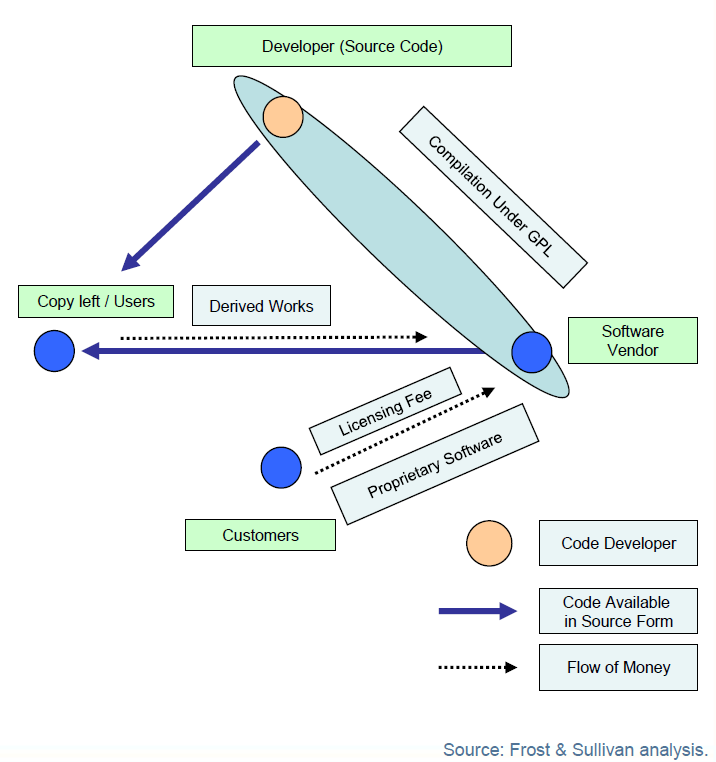
\includegraphics[width=.94\textwidth]{Impact-img1.png}}
%  \caption{The GPL Model}\label{fig:gpl-model}
% \end{figure}

% \begin{figure}[ht]\centering
%  \fbox{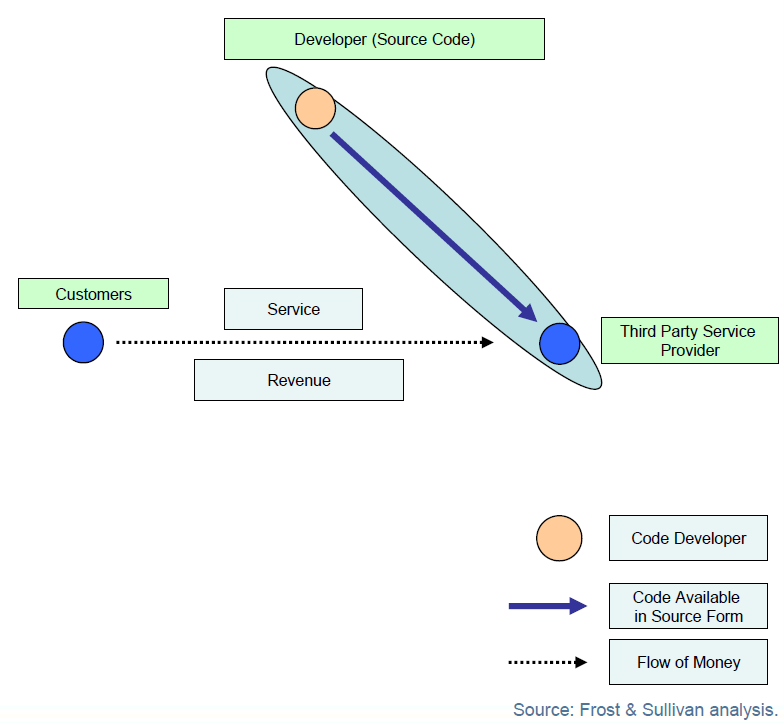
\includegraphics[width=.94\textwidth]{Impact-img2.png}}
%  \caption{The Third-Party Services Model}\label{fig:tps-model}
% \end{figure}

% \begin{compactenum}
% \item The \textbf{GPL model} (see Figure~\ref{fig:gpl-model}): With this model, the vendor
%   is required to make the new code available in source form but it can choose to keep the
%   new code as proprietary and charge for that proprietary software.  The vendor can
%   provide the code commercially as part of a larger platform (hardware/software product)
%   for which the companies receives revenue (license fee for the code + fees for technical
%   support, updates and upgrades).
% \item The \textbf{Third Party Service Model} (see Figure~\ref{fig:tps-model}) Many users
%   may be willing to employ a third party service for distribution, modifications
%   (debugging) and other support.
% \end{compactenum}

\eucommentary{
Where relevant, include information on how the participants will manage
the research data generated and/or collected during the project, in
particular addressing the following issues: What types of data will the
project generate/-collect? What standards will be used? How will this
data be exploited and/or shared/made accessible for verification and
re-use (If data cannot be made available, explain why)? How will this
data be curated and preserved?}

\TOWRITE{E.S. – Nicolas}{, ici je ne peux pas  écrire à ta place. Il faut juste que
tu répondes précisément aux questions posées ci-dessus.}

%Open source software.
%
%
%All software used and/or generated by the project will be Open Source.
%This is a deliberate choice of the project consortium, as commercial
%licenses (and patents) on this type of software only creates barriers
%in our scientific domain.
%
%Benefits of Open Source:
%
%Acquisition and Costs: lower costs, easy access to the infrastructure,
%lower risks of proprietary lock-in
%
%Flexibility: picking up from Open Source projects, reduces dependence on
%supplier, ability to view and modify the source code. Allows peer
%reviewed modifications, community discussions. Open Source provides the
%customer/end user the opportunity to innovate
%
%Support: from developer community.
%
%Besides being cost effective, Open Source software fosters
%reuse, reliability, flexibility, and interoperability.
%
%A consortium agreement will be established to manage ownership and
%access to key knowledge, including software generated by the project.

{\bf Open access policy and data protection.} OpenDreamKit will participate in the Open Research Data Pilot and is fully committed to ensure the open access of relevant project results and data. The consortium will comply with the Guidelines on Open Access to Scientific Publications and Research Data in Horizon 2020. 

The ambitious and interdisciplinary objectives of the project will result in the production of vast amount of research data (we refer to Figure \ref{fig:thebigpicture} and the corresponding subsection for more details). The primary results of the project are expected to take the form of an open-source software, which will be available through the project website and publicly available repositories. Moreover, as the project strives towards efficient integration and representation of various research data and reproducibility of the research results, which represents naturally a challenge, the project will generate a detailed description of the data sources with specifics pertaining to data management (metadata standards, policies for access and sharing and for reuse and distribution, plans for archival and preservation, with accompanying deadlines). This information will be presented in the Data Management Plan, to be delivered within the first six months after the project start and subsequently updated throughout. 

All scientific publications produced in the framework of the project will be either published in open access journals or self-archived using research data repositories. In addition, we will make all experimental data needed to reproduce/validate the results from scientific publications available through research data repositories (e.g. ZENODO, OpenAIRE). 

{\bf Intellectual Property Rights Management.} IPR management will be described in detail in the Consortium Agreement (CA), which will describe all issues regarding the IPR, confidentiality, know-how, rights on exploitation, the rights and obligations of the each partner. The CA will be prepared by the Coordinator, and then signed by all partners before the start of the project. 

Access rights to foreground and background needed for the execution of the project shall be deemed granted, on a royalty-free basis, as of the date of the grant agreement entering into force. Methodology, documents, know-how, software, and tools will be available to all in order to achieve the project objectives during the project lifetime. 

Most of the project results will have joint ownership due to a highly collaborative nature of the project. The CA will specify the terms of the resulting joint ownership, i.e., assignment of shares between joint owners, conditions of use, exploitation and management of jointly used IP. 

The CA will also outline rules for publication procedures to ensure that IP can be protected while minimising publication delay.

The costs related to IPR (including those related to protecting results) and dissemination (i.e., 'gold' open access publications) are included in the project budget of each participating organisation. 

\subsubsection{Communication Activities}
\label{subsubsect:communication}

\eucommentary{Describe the proposed communication measures for promoting the
project and its findings during the period of the grant. Where appropriate
these measures should include social media and public events with user
participation. Measures should be proportionate to the scale of the project,
with clear objectives. They should be tailored to the needs of various audiences,
including groups beyond the project's own community. Where relevant, include
measures for public/societal engagement on issues related to the project.}

Our intention is to increase the attractiveness of mathematics among young generation and females in particular as well as to improve the impact and maximise the visibility of the project activities on the entire VRE ecosystem. The following strategic access points will be used to maximise visibility:

\begin{compactenum}
\item An online presence that explains the OpenDreamKit concept and its applicability in layman's terms and offers significant information (website, social networks, Youtube, press releases).
\item Collaboration with other relevant European and national projects (existing and new ones). We refer to Section \ref{linked-projects} for more details on the linked research and innovation activities.  Presentation of the project results on the annual event 'Worldwide meetings of the free software.' 
\item Collaboration with European and national mathematical societies, e.g., European Mathematical Society, European Women in Mathematics.
\item Presentations/demonstrations at partner institution-specific, locally organised 'science holiday' and 'days of science'.
\item Popularisation papers and communication events addressed to people interested by ICT. 
\item Involvement in workshops / conferences on e-infrastructures and broad mathematical topics, e.g., Swiss Numerical Analysis Day.
\end{compactenum}
%%% Local Variables:
%%% mode: latex
%%% TeX-master: "proposal"
%%% End:

%  LocalWords:  eucommentary programme subsubsection tablehead longtable hline sur est
%  LocalWords:  e-infrastracture sémantique données amont j'ai mal si répond vraiment ce
%  LocalWords:  critère Systeme flushleft arraybslash Ergonomie il faut réflechir façon
%  LocalWords:  rendre l'outil attractif jeune génération génération des chercheurs va je
%  LocalWords:  définir donc terme Réfléchis possibilité tablettes mais aussi l'enseigner
%  LocalWords:  intéressante textgreater partie suivante demande elle ne serait mieux que
%  LocalWords:  unauthorised Maximise subsubsect organisational Pycon IPython Economie tu
%  LocalWords:  Standartisation Logiciel Libre includegraphics Impact-img1.png peux emph
%  LocalWords:  Impact-img2.png écrire répondes précisément posées ci-dessus TOWRITE fbox
%  LocalWords:  Simula Valeriya textwidth textwidth textbf compactenum longtable Jupyter
%  LocalWords:  organisation organise neighbouring Standartization programmes gpl-model
%  LocalWords:  tps-model thebigpicture Popularisation virtualised organisations Logilab
%  LocalWords:  organisations summarise organising capitalise realising minimising
%  LocalWords:  organised


\section{Update of the plan for exploitation and dissemination of result (if
    applicable)}
 Not applicable
 % Include in this section whether the plan for exploitation and dissemination of results
  % as described in the DoA needs to be updated and give details.

\section{Update of the Data Management Plan}

% Include in this section whether the data management plan as
% described in the DoA needs to be updated and give details.

A second version of the Data Management Plan was released in
\longdelivref{management}{data-plan2}. Up to minor updates to the list
of data sets, there was no change since
\longdelivref{management}{data-plan1}.


\section{Follow-up of recommendations Quality Management}

In this section, we will detail our actions in response to the recommendations and
comments of the reviewers and review the risk management and quality assurance procedures
adopted in in \pn project.

\section{Follow-up of recommendations and Quality Management}

In this section, we will detail our actions in response to the recommendations and
comments of the reviewers and review the risk management and quality assurance procedures
adopted in \pn.

\subsection{Follow-up of recommendations}

We are extremely grateful for the very constructive comments and
recommendations that were provided during the review itself and in the
formal report.

\newtheorem{recommendation}{Recommendation}{}

\begin{recommendation}
  A minor aspect: In the deliverable D5.11, authors have to clarify
  the reason why the speedup with the use of cores is not so high when
  you increment the number of cores. The presentation has also to be
  improved.
\end{recommendation}

Deliverable 5.11 was polished, complemented with a clarification and
resubmitted after the review.

\begin{recommendation}
  To include the KPIs in a centralized way in the technical report (KPI table)
\end{recommendation}

All KPI's are presented within a single section of the Technical
Report for reporting period. We tried making this section into a
table; however many of our KPI take the form of qualitative narratives
and do not fit well in such a table. Instead, we made individual
tables for each quantitative KPI.

\begin{recommendation}
  Demonstration of capabilities due to project results is crucial,
  especially for test cases/show cases. Often, such demonstrations are
  extremely technical. A higher level approach to such demonstrations
  is needed, so that potential users are not taken aback by the many
  actions they need to undertake. It would be good if the project team
  discusses this, and takes action to make demonstrations more
  attractive and appealing. This is also vital for the sustainability
  of the project results.
\end{recommendation}

We have discussed the matter within the project and we will be trying
our best during the next review. We are facing an intrinsic difficulty
due to OpenDreamKit's toolkit strategy. We indeed have a long
experience of delivering very progressive demonstrations at our
training workshops; in fact we often introduce some of the technology
stack even to hundreds of freshmen students at the occasion of our
classes. However much of that technology is not a single product of
OpenDreamKit per se. Rather it is an ecosystem of products, to which
OpenDreamKit makes many contributions. Often the contributions are by
nature almost invisible from the end-user perspective, and it takes
some technical context to highlight their relevance and impact on
usability or sustainability.

\begin{recommendation}
  Financial statements must be made available to reviewers no later
  than 15 days before Review Meeting in final form and to the
  Commission much earlier.
\end{recommendation}

Our previous project manager had left the project in August 2018, and
despite a rehiring process started as early as May 2018 the position
remained vacant until December 2018. We are happy to report however
that we very lucky in the recruitment. Our new project manager Izabela
Faguet -- together with the project coordinator -- took early and
active steps to devise, advertise, and enforce a strict time line to
ensure that all partners -- including UPSud itself -- would submit
their financial reports well on time.

\begin{recommendation}
  It is to be hoped that spend can be accelerated in the next year to
  make best advantage of the funds available and to ensure maximum
  benefit to the communities.
\end{recommendation}

On the day after the review a brainstorm was run among the
participants to explore opportunities of funds reallocation. Practical
feasibility was then explored and selection of best opportunities were
then discussed in the following weeks.

The largest source of tentatively unused funds was from Leeds,
following the departure to industry of its members. Most of the
resources ($\approx$180 k euros) were redistributed to the other partners.
This proved extremely useful to organize many additional dissemination
events -- making up for Leeds departure -- add a new case study
exploring the MitM approach in the context of proof systems, and
generally speaking increase the participant involvement on existing
tasks. This is formalized and explained in the 5th grant agreement
amendment.

Another source of tentatively unused funds was from \site{UK},
Indeed, those funds were originally reserved for the organization of
conferences early in the project which could finally be covered from
other sources. It was decided that \site{UK} would cover some of
the expenses ($\approx$60 k euros) for the organisation of our large
dissemination event at CIRM, enabling \site{PS} to reallocate funds
for other dissemination events.

\begin{recommendation}
  Greater attention must be paid to acknowledgement of EU funding in
  all areas. For exemple, include the name of the project in Software
  Carpentry: Related projects:
  \url{https://software-carpentry.org/join/projects/}
\end{recommendation}

We made sure that EU funding was acknowledged by the projects we
developed or contributed to:
\href{https://jupyter.org/about}{Jupyter},
\href{http://joommf.github.io/}{JOOMMF},
\href{https://www.gap-system.org/Contacts/funding.html}{GAP},
%\href{https://github.com/K3D-tools/K3D-jupyter}{K3D}
\href{https://linalg.org/support.html}{LinBox},
\href{https://pypersist.readthedocs.io/}{pypersist},
\href{https://mathhub.info/}{MathHub},
\href{https://gap-packages.github.io/Memoisation/}{Memoisation},
\href{http://www.mpir.org/news.html}{MPIR},
\href{https://uniformal.github.io//doc/}{MMT},
\href{https://pari.math.u-bordeaux.fr/funding.html}{PARI/GP},
\href{https://www.sagemath.org/development-ack.html}{SageMath},
\href{https://github.com/sagemath/sage-combinat-widgets}{Sage Combinat widgets},
\href{https://github.com/sagemath/sage-explorer}{Sage Explorer},
\href{https://github.com/nthiery/sage-gap-semantic-interface}{Sage GAP Semantic Interface},
\href{https://www.singular.uni-kl.de/index.php/background/funding.html}{Singular},
\href{https://ubermag.github.io/}{Ubermag}.

We have reached to Software Carpentry; their site is under
reconstruction and the aforementioned page is about disappear. We are
working with them for a proper location for the acknowledgment.
Presumably this will be on the pages of the lessons that ODK
contributed to.

We also asked the partners to double check their publications.

% https://github.com/gap-packages/Memoisation
% https://github.com/mtorpey/pypersist

\begin{recommendation}
  To develop a comic explaining the MitM approach.
\end{recommendation}
The comic has been published on:
\url{https://github.com/OpenDreamKit/OpenDreamKit.github.io/blob/master/public/images/use-cases/MitM.png}. It
has already been used in the MitM use case description at
\url{https://opendreamkit.org/2018/05/16/lmfdb-usecase/}, in conference presentations and
posters.

\begin{recommendation}
  To disseminate the Adoption by Logipedia of the MitM principle of
  integrating (logical) systems by aligning concepts.
\end{recommendation}
We have made a blog post about this, see \url{https://opendreamkit.org/2019/01/24/logipedia/}.

\begin{recommendation}
  Some guidelines (set of recommendations) for using the different
  tools provided by OpenDreamKit would be recommendable.
\end{recommendation}
We have expanded our use case section on \url{opendreamkit.org} and
will keep doing so.

% , and
% wrote additional blog posts, notably on how to deploy custom VRE's; see e.g.
% \url{https://opendreamkit.org/2018/10/17/jupyterhub-docker/}.

\begin{recommendation}
  Some guidelines (set of recommendations) for using the different
  hardware architectures would be recommendable.
\end{recommendation}

\ednote{@ClementPernet: hardware architecture recommendations}

%%% Local Variables:
%%% mode: latex
%%% TeX-master: "report"
%%% End:

%  LocalWords:  newenvironment noindent textbf begingroup endgroup delivref emph WPref
%  LocalWords:  ipython-kernels specialized longlocaltaskref dissem hpc optimization
%  LocalWords:  MPIRsuperoptimiser parallelization sage-HPCcombi XKaapi OmpSS
%  LocalWords:  vectorization localtaskref sage-paral-tree

\subsection{Risk management}
\ednote{This whole section seems to be about RP2}
\subsubsection{Recruitment of highly qualified staff}
Recruitment of highly qualified staff was planned to be a high risk
when the Proposal was written. And unfortunately it turned out we were
right. In such a field as computer science and software development,
potential candidates who are likely to be fairly young considering
only temporary positions are offered, are very scarce. Furthermore
they need to make a choice between public and private bodies which are
very attractive, and the choice between pure development and research.
Because of this difficulty to recruit in the past year, there have
been slight changes in the workplan, which do
not put the project results at risk.

The following people were hired in the past year or are in the hiring pipeline for next year\\
\begin{tabular}{|l|c|r|r|r|}\hline
  NAME&GENDER&PARTNER&POSITION&HIRING DATE\\\hline
  Theresa Pollinger & F & \site{FAU} & Junior Researcher & October 2017\\
  Tom Wiesing & M & \site{FAU}  & Junior Researcher & September 2017\\
  PD. Dr. Florian Rabe & M & \site{FAU}/\site{PS} & PostDoc & December 2017\\
  Dr. Katja Ber\v{c}i\v{c} & F & \site{FAU} & PostDoc &  November 2018\\
\hline
\end{tabular}\\
~\\
Dr. Florian Rabe is a joint appointment and splits his time and research between \site{FAU} and \site{PS}, which reflects
the close cooperation and cross-fertilization of methods in \WPref{dksbases}. 

\ODK partners had to face some Human Resources issues; this mostly
concerned Reporting Period 1 where most of the hiring occurred, with
reduced effects on Reporting Period 2:
\begin{itemize}
\item{\site{PS}:}
  Thanks to an early start in the recruitment process, and despite
  some difficulties in attracting experienced candidates for a part
  time position, the project manager position (24PM) was filled by
  Benoît Pilorget shortly after the start of the project. Unfortunately at month 36 the project
finds itself without a Project manager since the departure of B. Pilorget.

  The recruitment of \site{PS}'s first Research Engineer (48PM) was
  delayed by four months because the top ranked candidate for this
  position, Erik Bray, was originating from the US and needed time to
  arrange for his moving; there were also some administrative delays
  (visa, ...).

  The second Research Engineer position (36PM) was more problematic
  for internal administrative reasons. The top ranked candidate,
  Jeroen Demeyer, had the perfect profile; however for family reasons,
  he wished to work most of the time from Ghent in Belgium. After eight
  months investigating an administrative solution to hire him at
  \site{PS}, and a temporary four month solution, it was decided with
  OpenDreamKit's Steering Committee and Project Officer to instead add
  Ghent's university as new partner, hire Jeroen Demeyer there, with an
  adequate budget transfer and amendment to the Grant Agreement.

  Those delays have induced late start on several tasks, and costed
  much management time. However the excellence of the recruitment,
  well confirmed by the results obtained so far, was worth it and soon
  compensated for the late start.

  In addition to this, a three year PhD position was open to work on
  WP6, starting from Month 12. By lack of suitable candidate, this
  position was converted into a PostDoc position; this position was
  filled in half by Florian Rabe in Spring 2018. A research software
  engineer, Odile Benassy was hired in June 2018 until the end of the
  project using the remaining PMs.\\

\item{CNRS:} Because the research engineer offer (48PM) was still not
  filled in the Summer 2016, the CNRS decided to divide the position
  in two full positions of 24 PM each. As a result, a candidate was
  selected for one of the two positions and began his work in Fall
  2016. Thanks to the PM division, there should be no delay in any
  task or
  deliverable. \\

\item{JacobsUni:} Michael Kohlase, lead PI for Jacobs University, has
  moved on 01/09/2016 to Friedrich-Alexander-Universität
  Erlangen-Nürnberg, and most of his team will follow him. The necessary changes have been
  implemented in a grant agreement amendment in 2017.\\

\item{UJF:} The original tentative candidate for UJF's Research
  Engineer position (12PM, planned to start on Month 1), Pierrick
  Brunet, finally declined the position to accept an alternative
  permanent offer. The position was filled by another candidate in
  Autumn 2016. This induced a delay of Deliverable \textbf{D5.2} from Month 12
  to Month 18, without impact on other tasks.\\

\item{UNIKL:} UNIKL had to split the 12 PM planned for a software developer into 2 shorter positions (Anders Jensen and Alexander Kruppa) in order to deliver the planned work on time. Indeed the few qualified persons for this job were not able to accept this 12 months position during the timelapse planned within the project.\\

\item{USFD:} The University of Sheffield has also been struggling in
  the hiring process of a postdoc (36PM), and a move of the PI to the
  University of Leeds.\\

\item{Southampton:} Southampton faced administrative difficulties in
  the recruitment of Marijan Beg (38PM) as a post-doc, due to
  Marijan's Croatian nationality and recent changes in the relevant
  legislation. His recruitment was delayed by four months, and
  therefore some tasks and deliverables were postponed. We will
  compensate for the delay by putting more staff effort in at later
  stages in the project. We don’t expect any delay nor implication on
  the main tasks of OpenDreamKit.

\item{UVSQ:} Nicolas Gama was on a long-term leave until September
  2017. This did not affect the project in any way.\\

\item{UZH:} The University of Zürich partner is only composed of one
  person, Paul-Olivier Dehaye, who does not enjoy a permanent position
  there. There have been worries that Mr Dehaye's contract with his
  university might end earlier than planned within OpenDreamKit. But
  thanks to the action of the OpenDreamKit steering committee, Mr
  Dehaye has been technically rehired by UZH as a scientific
  consultant until the end of the planned implication.\\

\item{Simula:} Everything is fine concerning temporary staff
  recruitment on the Simula side, however we have had to endure the
  hazards of human ressources with Hans-Peter Langtanger (the PI when
  the Grant was signed) being on a long-term sick leave, and with
  Martin Alnaes replacing him as PI having a paternity leave. However
  Benjamin Ragan-Kelley has stepped in to lead the
  Simula contribution in the meantime and all planned tasks are on time.\\
\end{itemize}


Altogether, this confirmed that the recruitment of highly
qualified staff is indeed a risky endeavour, which induced delays on
several deliverables. However the planned mitigation measures --
taking into account the pool of potential candidates in the design of
the positions, aggressive advertisement, weak coupling between tasks
-- worked adequately: with appropriate reshuffling of the work plan,
this did not impact the overall progress of the project.

\subsubsection{Different groups not forming effective team}

As expected, this risk was tamed by the existence of many preexisting
collaborations between the partners and of ``joint itches to scratch
together'' (to use a common open source software metaphor). The
organization of many joint workshops (for example the Sage-GAP
workshop, the Atelier Pari attended by SageMath developers, the WP6
workshops) helped bootstrap joint activities through brainstorms and
coding sprints. Upcoming workshops are planned on Year~2 to strengthen
collaborations with the social aspects team in Oxford and the Singular
team in Kaiserslautern.


\subsubsection{Implementing infrastructure that does not match the needs of end-users}

The consortium is keeping in their minds the end-user needs. Since
OpenDreamKit is improving already existent software which have their
own users, their needs are naturally met. However Key performance
Indicators will evaluate the effects of OpenDreamKit on these
software. KPIs, indicated in the Proposal, will be launched this
Autumn with the help of the end-user group which was merged with the
Advisory Board. Constant links between the accomplished work and the
end-user needs should be made in WP2 deliverables and also in WP7
deliverables when relevant.  Open tracking of KPIs evolution can be
found on
\href{https://github.com/OpenDreamKit/OpenDreamKit/labels/KPI}{GitHub}.

\subsubsection{Lack of predictability for tasks that are pursued jointly
  with the community}

As planned, we are regularly shifting manpower around to adapt for the
variability of the involvement of the community in the different
tasks. For example, the SageMath Jupyter kernel of
\longdelivref{UI}{ipython-kernels-basic} was mostly implemented by the
community which allowed to focus on other tasks such as the long term
task~\longdelivref{component-architecture}{portability-cygwin}.  On
the other hand many other deliverables were implemented with very
little help from the community.

\subsubsection{Reliance on external software components}

There is not much to report on this front yet: none of the external
software component we rely on have failed us. Quite on the contrary,
critical software like \Jupyter have continued to blossom. Besides the
high modularity of the design means few components are critical to the
overall success of the project.

%%% Local Variables:
%%% mode: latex
%%% TeX-master: "report"
%%% End:

%  LocalWords:  hline cross-fertilization WPref dksbases Pilorget Pierrick textbf Kruppa
%  LocalWords:  Dehaye Dehaye's Dehaye Alnaes organization Jupyter longdelivref Benassy
%  LocalWords:  ipython-kernels-basic portability-cygwin subsubsection

\subsection{Quality assurance plan}
\label{section.QAP}

\subsubsection{Deliverables quality: Quality Review Board}

The Quality Review Board is the Consortium Body that fosters best
possible quality in the delivered work of the project.
All four members of the board
have a research interest in the quality of software in computational
science, and use and share their experience to benefit the quality of
the work.

The board was chaired by Hans Fangohr, from the University of
Southampton and European XFEL GmbH (Germany). He is supported in this task by
Mike Croucher from the University of Leeds and now
Numerical Algorithm Group (UK), Alexander Konovalov from
the University of St Andrews (UK), and by Konrad Hinsen from the Centre de
Biophysique Moléculaire (France) with whom a Non-Disclosure Agreement was
signed.

These board members engage with European initiatives working towards
improvement of the software quality in research, in particular in
computational and data science; both as voluntary activities and key
of their professional roles. Mike Croucher was the head of research
computing at Leeds, and is well known through his outreach blog; Alexander Konovalov
is a fellow of the Software Sustainability Institute and an active
member of the Software Carpentry community; Konrad Hinsen has
founded and is editing the ReScience Journal for reproducible Science,
and Hans Fangohr is the founder of the UK's only centre for
doctoral training in computational modelling with focus on software
engineering training for scientists, a fellow of the Software
Sustainability Institute, was chairing the EPSRC's national scientific
advisory committee on high performance computing, is heading
data analysis infrastructure development at the European XFEL research
facility, and leading the data analysis work package in the Photon and
Neutron Open Science Cloud H2020 project that works towards
implementation of the European Open Science Cloud.

The quality review board has reviewed deliverables after the reporting
period 1 and 2, identified good practice - both in terms of software
engineering content but also presentation of the work -, produced
reports, and shared the findings with all members in the project to
improve the quality of the remaining deliverables. An improvement of
the quality of deliverable reports at the end of reporting period 2 in
comparison to reporting period 1 was noted. The reports are available
on request. The board has stuck to its no-blame
culture in its reporting, but has pointed out deliverable reports of
very high quality.



\subsubsection{Infrastructure quality: End-user group}


It was decided by the Steering Committee during the
\href{http://opendreamkit.org/meetings/2015-09-02-Kickoff/management_structure/}{kick-off
  meeting} to slightly modify the management structure by having only
one gender-friendly Advisory Board composed of 6 people (as agreed a
few months later at the
\href{http://opendreamkit.org/meetings/2016-06-27-Bremen/minutes/}{Bremen
  meeting}), some of which to be end-users.

Members of the board are: Jacques Carette from the McMaster University, Istvan Csabai from the Eötvös University Budapest,
Françoise Genova from the Observatoire de Strasbourg, Konrad Hinsen from the Centre de Biophysique Moléculaire,
William Stein who is CEO of SageMath, Inc. (SME), and Paul Zimmermann from INRIA.

%%% Local Variables:
%%% mode: latex
%%% TeX-master: "report"
%%% End:

%  LocalWords:  subsubsection Dissemmination ldots sec:orgc218a3a
%  LocalWords:  github Csabai


\section{Deviations from Annex 1 (if applicable)}
  % Explain the reasons for deviations from the DoA, the consequences and the proposed
  % corrective actions

There was no major deviation from Annex 1. All deliverables due for M18 were delivered
  within the timeframe of the 1st Reporting Period, and all milestones in this period were
  reached.  Slight modifications were brought to \WPref{hpc} and \WPref{dksbases} and were
  included in the AMD-676541-13.

\subsection{Tasks}
% Include explanations for tasks not fully implemented, critical objectives not fully
% achieved and/or not being on schedule.  Explain also the impact on other tasks on the
% available resources and the planning

No deviation from the tasks. All workplan is on time at the end of the Reporting
Period.

However, there were four deliverables that
were handed in late. We will explain the situation and implications in
each case. Therefore, administratively speaking, Milestone 2
(Implementations), originally due on Month 24, was only reached in
Month 36, though with little, if any, consequences on the project as a
whole.

\subsubsection{\protect\delivtref{dissem}{ils-tool}}
This deliverable, a tool for publishing and organizing curated
collections of Jupyter notebooks, was delivered in month 36, a delay
of 12 months after the initially planned schedule.

The initial plan had been to build upon an already existing prototype,
whose development had started at a \Sage meeting back in 2015. The
original tool was specific to \Sage, but broader in scope and not tied
to Jupyter. Given the constantly evolving context, it quickly became
apparent that this tool did not properly address the community needs.
We thus took on evaluating other available open source solutions,
which considerably delayed the deliverable.

As we were not able to find an appropriate solution to build upon, we
finally decided to bootstrap a new project, called
\emph{planetaryum}. Once the development of \emph{planetaryum}
started, we were able to complete the version 0.1 in the planned
time frame.

Since other solutions were available before \emph{planetaryum}, albeit
less powerful, the delay in the deliverable did not impact other tasks
in the project.


\subsubsection{\protect\delivtref{UI}{ipython-kernels}}

This deliverable of full-featured kernels for GAP, Pari, Singular, etc.  has been
delivered in month 36 after a delay of 12 months.  The initial plan was for delivery in
Month 24, but was delayed to ensure a high quality of the delivered software, as more
time-sensitive resources were directed away from this task during months 12-24.  The delay
had no impact beyond the deliverable itself, as no other tasks relied strongly on this
deliverable being ready, and the result is a much stronger collection of Jupyter kernels
for mathematical software.

\subsubsection{\protect\delivtref{UI}{sage-sphinx}}

This deliverable is delivered in month 36, a delay of 12 months after the initial schedule
of month 24.  Progress was slower than planned, due to the nature of coordinating with
large software collaborations.  Additionally, work was shifted to other tasks during early
stages, resulting in the delay of this deliverable.  There have been no negative
consequences of the delay, as its delivery was not a prerequisite for other tasks.  As a
result of the delay, we have delivered much greater work than initially planned, including
significant improvements to the Sphinx documentation system itself used by projects all
over the world, and an Enhancement Proposal to improve the Python language itself,
ensuring wide impact for this work.


\subsubsection{\protect\delivtref{dksbases}{psfoundation}}
This deliverable report was delayed, as we found it useful to extend the scope of the work
reported from just the format of the interface theories and aligments -- these are
extensively discussed in the report as well -- to a full account of the Math-in-the-Middle
interoperability paradigm for \pn and discuss two full-scale use cases. It just made more
sense to deliver this report together with D6.8 (the resources for the use cases) for
Milestone M9 \emph{First Math-In-The-Middle-based interoperability prototype} in month 36,
in particular, since the delay of D6.5 did not delay the research and development in WP6
(after all, an earlier version of much of the content of D6.5 has been pre-published
as~\cite{WieKohRab:vtuimkb17,KohMuePfe:kbimss17} near the original deadline of D6.5 and
was therefore available to the \pn partners). 

This way D6.5 can serve as as reference for opening the MitM paradigm to outside users. We
are currently working on a high-visibility Journal publication based on D6.5 and D6.8
(presumably Journal of Symbolic Computation). 

\subsection{Use of resources}
% Include explanations on deviations of the use of resources between actual and planned
% use of resources in Annex 1, especially related to person-months per work package.

All changes of use of resources were included in the two amendments previously cited and were
due to modifications in the personnel. Those adjustments were due to the change of positions
of some key \ODK participants and expected difficulties in hiring planned
staff. The work plan has been updated accordingly, with no foreseeable
impact on the achievement of tasks, deliverables, and milestones.

Another minor deviation in the proposed use of resource was that FAU hired students to do
some routine jobs (simple formalizations, and the creation of alignments in WP6 and the
creation of example documents in WP4) that did not require the attention of a mature
researchers. As the pay grade of student assistant is roughly 1/4 of that of full
researchers, this action was cost-effective. An unplanned effect was that the reported
person months went up considerably, exceeding the planned amount, without incurring
additional cost. 

\subsubsection{Unforeseen subcontracting (if applicable)}

Not applicable.
% Specify in this section: a) the work (the tasks) performed by a subcontractor which
  % may cover only a limited part of the project; b) explanation of the circumstances
  % which caused the need for a subcontract, taking into account the specific
  % characteristics of the project; c) the confirmation that the subcontractor has been
  % selected ensuring the best value for money or, if appropriate, the lowest price and
  % avoiding any conflict of interests

\subsubsection{Unforeseen use of in kind contribution from third party against payment or
  free of charges (if applicable)}

 Not applicable. 
 % Specify in this section: d) the identity of the third party; e) the resources made
  % available by the third party respectively against payment or free of charges f)
  % explanation of the circumstances which caused the need for using these resources for
  % carrying out the work.

\printbibliography

\end{document}

%%% Local Variables:
%%% mode: latex
%%% TeX-master: t
%%% End:

%  LocalWords:  maketitle githubissuedescription newpage newcommand xspace Jupyter dissem
%  LocalWords:  tableofcontents visualizations composability itemize analyzed taskref hpc
%  LocalWords:  dissemination-of-oommf-nb-virtual-environment taskref dissem taskref pn
%  LocalWords:  dissemination-of-oommf-nb-workshops dissem ibook taskref taskref taskref
%  LocalWords:  oommf-python-interface oommf-py-ipython-attributes taskref oommf-nb-ve
%  LocalWords:  oommf-tutorial-and-documentation taskref oommf-nb-evaluation taskrefs
%  LocalWords:  delivref pythran-typing sage-paral-tree subsubsection organized Dagstuhl
%  LocalWords:  co-organized organization modularization ipython-kernels nbdime Pythran
%  LocalWords:  jupyter-collab ystok WPref dksbases compactitem emph WPtref DehKohKon
%  LocalWords:  iop16 textbf tasktref lfmverif triformal formalized biformal ossp09 Dima
%  LocalWords:  hline Marijan Pilorget Pierrick Kruppa Dehaye Dehaye's Dehaye's Alnaes
%  LocalWords:  Konovalov Hinsen github printbibliography enlargethispage
